% 	This template is  MIT licensed.

% 	Basic file to demonstrate the usage of this LaTeX template.
% 	You can build your own paper/thesis on top of this file.
% 	Simply adjust the document class and all metadata and start working.
%
\documentclass[
	language=english, % set to english or german
	type=master, % set to bachelor, master or seminar
    13pt
]{isthesis}

\usepackage{lipsum}
\linespread{1.5} % Line spacing

\usepackage[utf8]{vntex}

% custom package
\usepackage{eurosym}
\usepackage{makecell}
\usepackage{hyperref}
\usepackage[utf8]{inputenc}
\usepackage{tabto} 
\usepackage{longtable}
\usepackage{algorithm} 
\usepackage{algpseudocode}
\usepackage{biblatex} %Imports biblatex package
\usepackage{svg}
% \usepackage{multirow}
% \usepackage{floatrow}

% Graphics rendering using TikZ
% See: https://en.wikibooks.org/wiki/LaTeX/PGF/TikZ
\usepackage{tikz}
\usepackage{xcolor}
\definecolor{light-gray}{gray}{0.95}
\newcommand{\code}[1]{\colorbox{light-gray}{\texttt{#1}}}
% Include required TikZ libraries here, some exemplary libraries are pre-included
\usetikzlibrary{calc}
\usetikzlibrary{matrix}
\usetikzlibrary{positioning}
\usetikzlibrary{shapes.geometric}

\usepackage{amsthm}
% \usepackage{ntheorem}
\newtheoremstyle{theoremst}% name of the style to be used
  {\topsep}% measure of space to leave above the theorem. E.g.: 3pt
  {\topsep}% measure of space to leave below the theorem. E.g.: 3pt
  {\normalfont}% name of font to use in the body of the theorem
  {0pt}% measure of space to indent
  {\bfseries}% name of head font
  {:}% punctuation between head and body
  { }% space after theorem head; " " = normal interword space
  {\thmname{#1}\thmnumber{ #2}\textnormal{\thmnote{ (#3)}}}

\newtheoremstyle{examplest}% name of the style to be used
  {\topsep}% measure of space to leave above the theorem. E.g.: 3pt
  {\topsep}% measure of space to leave below the theorem. E.g.: 3pt
  {\normalfont}% name of font to use in the body of the theorem
  {0pt}% measure of space to indent
  {\bfseries}% name of head font
  {\\}% punctuation between head and body
  { }% space after theorem head; " " = normal interword space
  {\thmname{#1}\thmnumber{ #2}\textnormal{\thmnote{ (#3)}}}


% \theorembodyfont{\normalfont}
% \theoremseparator{:}
\theoremstyle{theoremst}
\newtheorem{definition}{Định nghĩa}[section]
\newtheorem{theorem}{Định lý}[section]
\newtheorem{proposition}{Khẳng định}[section]

% \theoremstyle{break}
% \theorembodyfont{\normalfont}
\theoremstyle{examplest}
\newtheorem{remark}{Nhận xét}[section]
\newtheorem{example}{Ví dụ}[section]

% \theoremstyle{remark}
% \newtheorem*{remark}{Remark}

%Add your library here
\addbibresource{refs.bib}

% Import acronyms
\input{config/acronyms}

% Import symbols
\input{config/symbols}

% Import custom commands
\input{config/commands}

% Import custom code block
\input{config/code_block.tex}

% Document meta information
\isthesis{
    title={LUẬN VĂN THẠC SĨ},
    sub-title={PHƯƠNG PHÁP TÌM KIẾM LÂN CẬN RỘNG THÍCH ỨNG \\ CHO MỘT SỐ LỚP BÀI TOÁN ĐỊNH TUYẾN PHƯƠNG TIỆN},
    author-name={Nguyễn Mạnh Linh}, 
    % Separate multiple authors with commas
    % author-email={linhnguyen.code@gmail.com},
    % author-matriculation={MATRICULATION NUMBER},
    % author-phone={+49 XXXXXXXXX}, % Use international numbers format
    % author-address={STREET},
    % author-zip={ZIP},
    % author-city={CITY},
    principal-supervisor={TS. Hoàng Nam Dũng}, % This must be a professor
    % associate-supervisor={SUPERVISOR}, % This is your main supervisor, i.e., a post doc or doctoral student
    tutor-supervisor={}, % If required, define an additional supervisor resp. tutor here
    group-institute={Trường Đại học Khoa học Tự nhiên},
    % group={Image Data Exploration and Analysis (IDEA) Lab},
    % studies={M.Sc. International Information Systems}, %your field of studies, i.e. Wirtschaftsinformatik or International Information Systems
    %
    %associate-group={}, % When the thesis is done in cooperation with another chair, add it here
    %associate-group-institute={}, % add cooperating institute or university here
    seminar={SEMINAR}, % The title of your seminar
    submission-date={2023-11-01}, % The date you handed in your document: Format yyyy-mm-dd
    primary-logo={assets/hus.png}, % Uses the FAU logo by default
    %primary-logo-height={}, % Uses 16mm as default height
    %secondary-logo={}, % Logo of the secondary institution (cooperating chair/university), USES Faculty logo by default
    %secondary-logo-height={} % Uses 16mm as default height
}


\begin{document}
    % Title page
    \newcounter{savepage}
    \maketitle

	% Quote
    % You can put an optional quote page in front of your content
    %   \quotepage[author={Arthur C. Clarke}]{
    %   	        Any sufficiently advanced technology is indistinguishable from magic.
    %   }
    
    % Table of contents
    \tableofcontents

    % \begin{abstract}
   Trong luận văn này, tác giả nghiên cứu mô hình toán học cho lớp các bài toán định tuyến xe (\textit{Vehicle Routing Problem} - VRP). Các thuật toán liên quan được giới thiệu và phân loại xuyên suốt lịch sử hơn $60$ năm phát triển của VRP. Tác giả tập trung vào thuật toán \textit{Tìm kiếm lân cận rộng thích ứng} (\textit{Adaptive Large Neighborhood Search}) để giải bài toán \textit{Định tuyến xe với ràng buộc khung thời gian} (\textit{Vehicle Rouing Problem with Time Window - VRPTW}). Một thuật toán hủy mới được tác giả phát triển giúp giảm nhanh số xe sử dụng. Thêm vào đó, tác giả đề xuất một hiệu chỉnh cho ALNS được gọi là B-ALNS (\textit{Boosted - Adaptive Large Neighborhood Search}). Các thuật toán được đánh giá trên các tập dữ liệu với số lượng yêu cầu từ nhỏ ($100$ yêu cầu) tới rất lớn ($1000$ yêu cầu). B-ALNS được chỉ ra có hiệu năng vượt trội so với ALNS (lên tới hơn $30\%$) và tiết kiệm tới $75\%$ tài nguyên tính toán cho một số cấu hình trong khoảng thời gian nhất định. Ngoài ra, tác giả đưa ra gợi ý áp dụng ALNS, B-ALNS cho các tình huống thực tế với mục đích khác nhau.
\end{abstract} 

    

    % \begin{abstract}
	%     % Add your abstract here:
        
	% 	% \lipsum[1]
	% \end{abstract}

    % List of figures (if you have figures)
    % \listoffigures

    % List of tables (if you have tables)
    % \listoftables
    
    % List of listings (if you have listings)
	% \lstlistoflistings

    % List of abbreviations (if you use acronyms)
    %\listofabbreviations

    % List of symbols (if you use symbols)
    %\listofsymbols
	
	% Abstract
	%
	% Comment out this part, if you don't require an abstract

	
	% storing the last pagenumber
    \setcounter{savepage}{\value{page}}
    
    
    % Content
    \begin{content}
        % Add your content files:
        \chapter*{Mở đầu}
\label{chap:introduction}
\addcontentsline{toc}{chapter}{Mở đầu}

Từ xưa tới nay, giao vận luôn là một trong những ngành đóng vai trò quan trọng trong nền kinh tế. Giao vận và quản lý chuỗi cung ứng đóng vai trò là một cầu nối giữa các đơn vị sản xuất và người tiêu dùng. Nó cũng là một trong những ngành có ảnh hưởng lớn đến sự phát triển của một quốc gia. 

Từ những thập niên 90 của thế kỉ trước, thời kì bùng nổ của Internet đã thúc đẩy một hình thức bán hàng hoàn toàn mới, đó là bán hàng trực tuyến. Hàng loạt các sàn thương mại điện tử lớn ra đời, có thể kể đến như Amazon (Mỹ - 1994), Alibaba (Trung Quốc - 1999), Rakuten (Nhật Bản - 1997). Ngày nay các sàn thương mại điện tử này trở thành những công ty hàng đầu thế giới không chỉ ở lĩnh vực bán hàng mà là cả công nghệ. Việc phát triển vũ bão của các sàn thương mại điện tử dẫn đến số lượng hàng hóa được tiêu thụ trên toàn cầu tăng lên một cách đáng kinh ngạc so với bán hàng truyền thống. Logistic và quản lý chuỗi cung ứng là một trong những xương sống của thương mại điện tử cùng với \textit{nền tảng công nghệ}, \textit{nền tảng thanh toán} hay \textit{chăm sóc khách hàng}... Để quản lý, giao vận số lượng đơn hàng lớn như vậy tới tay khách hàng, cách thức làm việc trong ngành logistic cũng phải thay đổi rất nhiều, áp dụng những công nghệ hiện đại hơn cách làm truyền thống.

Một trong những bài toán quan trọng nhất của logistic là bài toán vận tải hay định tuyến xe (hay người giao hàng). Với lượng xe có tải trọng hữu hạn, chúng ta cần định tuyến các xe này để giao hàng cho khách hàng ở các địa điểm khác nhau từ kho. Mục tiêu là tối ưu tổng quãng đường di chuyển của tất cả các xe để giảm chi phí vận hành. Lớp bài toán như vậy được gọi là \textit{Vehicle Routing Problem - VRP}. Phiên bản đơn giản của VRP là TSP (\textit{Travelling Salesman Problem}) hay bài toán người đưa hàng. Trong TSP, chúng ta có một người đưa hàng cần đi qua tất cả các địa điểm để giao hàng và quay trở về điểm xuất phát. TSP hay VRP là nhóm bài toán NP-hard, hiện tại người ta vẫn chưa tìm được lời giải chính xác trong thời gian đa thức. Tuy nhiên, với sự phát triển của các thuật toán hiện đại, chúng ta có thể tìm được nghiệm "gần" tối ưu cho nhiều bài toán NP-hard (có kích thước lớn) với chất lượng tương đối cao trong thời gian hợp lý.

VRP lần đầu tiên được giới thiệu bởi Dantzig, George B, Ramser và John H \cite{dantzig1959truck}, rất sớm trước thời kì bùng nổ Internet những năm 90! Tuy nhiên, cho tới nay, VRP vẫn thu hút được sự quan tâm lớn từ cộng đồng những nhà toán học hay khoa học máy tính bởi tính ứng dụng cao của nó. Với nhu cầu giao vận cùng lượng khách hàng cần phục vụ ngày càng tăng của các doanh nghiệp, việc tối ưu hóa chi phí vận hành là một vấn đề cấp thiết. Nhiều doanh nghiệp đã ứng dụng việc định tuyến tự động thay vì để tài xế tự tìm đường thủ công khi giao hàng như trước đây, thế nên việc tìm ra các tuyến đường "gần" tối ưu cần diễn ra nhanh chóng để tránh người giao hàng, hay lái xe phải chờ lâu để có được lộ trình cần thiết trước khi thực hiện giao hàng. 

Trong luận văn này, tác giả nghiên cứu mô hình toán học của VRP cùng các biến thể của nó và các thuật toán giải quyết bài toán này. Tác giả sử dụng thuật toán ALNS (\textit{Adaptive Large Neighborhood Search - S. Ropke và D. Pisinger} \cite{ropke2006adaptive}) làm thuật toán cơ sở cho các thực nghiệm. ALNS được phát triển dựa trên LNS - \textit{Large Neighbourhood Search - Shaw \cite{shaw1997new} \cite{shaw1998using}}. Hiệu năng và chất lượng nghiệm của ALNS được đánh giá trên các tập dữ liệu thực tế với số lượng yêu cầu (khách hàng) từ nhỏ tới rất lớn. Tác giả đề xuất một thuật toán hủy mới cho ALNS gọi là \textit{Xóa tuyến tệ} (\textit{Bad Route Removal}) giúp giảm số xe sử dụng một cách nhanh chóng. Thêm vào đó, tác giả cũng đề xuất một hiệu chỉnh cho việc tự động điều chỉnh trọng số lựa chọn thuật toán trong ALNS giúp tăng hiệu năng và tiết kiệm tài nguyên so với ALNS gốc một cách đáng kể, thuật toán được đặt tên là B-ALNS (\textit{Boosted - Adaptive Large Neighborhood Search}). Trong thực nghiệm với tập dữ liệu rất lớn với $1000$ yêu cầu, B-ALNS tiết kiệm đến $75\%$ tài nguyên so với ALNS gốc, khi sử dụng cùng một lượng tài nguyên, B-ALNS đạt được kết quả tốt hơn ALNS gốc đến $30\%$ trong thời gian chạy ban đầu của thuật toán.

\begin{figure}[H] % places figure environment here   
  \centering % Centers Graphic
  \includegraphics[width=0.9\textwidth]{figures/routes_c101.png} 
  % \includesvg[scale=1]{figures/core-object}
  \caption{VRP với 10 xe phục vụ 100 khách hàng (cấu hình Solomon C101).} 
  % \label{fig:fg_02}
\end{figure}

Các vấn đề được đề cập trong luận văn này được trình bày trong 4 chương. \hyperref[chap:introduction]{Phần mở đầu} giới thiệu vấn đề nghiên cứu. \hyperref[chap:model]{Chương 1} phân loại các biến thể của VRP và đưa ra các định nghĩa cũng như mô hình toán học của chúng.
\hyperref[chap:solution]{Chương 2} giới thiệu khái quát một số  phương pháp giải quyết VRP đã được nghiên cứu trước đó.
\hyperref[chap:search]{Chương 3} trình bày phương pháp tìm kiếm lân cận rộng và thuật toán tìm kiếm lân cận rộng thích ứng. Ngoài ra, \hyperref[chap:search]{chương 3} cũng đưa ra cấu trúc chương trình và các lớp chính được sử dụng để triển khai thuật toán tìm kiếm lân cận rộng thích ứng giải VRP với ràng buộc khung thời gian.
\hyperref[chap:experiment]{Chương 4} trình bày kết quả thực nghiệm và đánh giá hiệu năng của thuật toán.
\hyperref[chap:conclusion]{Phần kết luận} tóm tắt lại các kết quả đạt được và đề xuất hướng phát triển trong tương lai.

        \chapter{Định nghĩa và một số kí hiệu}
\label{chap:model}

Trong chương này, chúng ta sẽ đưa ra định nghĩa chính tắc cho lớp các bài toán định tuyến xe. Các định nghĩa này được xây dựng theo ngôn ngữ của lý thuyết đồ thị được đưa ra bởi Toth (2002) \cite{toth2002vehicle}. 

Các bài toán được mô tả thuộc lớp VRP (\textit{vehicle routing problem}) bao gồm \textit{định tuyến xe với ràng buộc tải trọng} - CVRP (\textit{capacited VRP}), \textit{định tuyến xe với ràng buộc khung thời gian} - VRPTW (\textit{VRP with time windows}), \textit{định tuyến xe với lấy và giao hàng} - VRPPD (\textit{VRP with pickup and delivery}).

\begin{figure}[H] % places figure environment here   
  \centering % Centers Graphic
  \includegraphics[width=0.8\textwidth]{figures/vrp.png} 
  \caption{Các bài toán, biến thể của VRP} % Creates caption underneath graph
  \label{fig:fg_01}
\end{figure}

\section{Định nghĩa bài toán}
\label{sec:def}

\subsection{CVRP}

Trước hết ta xem xét mô hình cho bài toán \textit{nguyên bản}: \textit{bài toán định tuyến xe với ràng buộc tải trọng}. Một cách tự nhiên, tại sao không phải là VRP (không ràng buộc)? Bạn sẽ thấy rằng nếu không có bất kì ràng buộc nào thì một xe có thể phục vụ tất cả các yêu cầu và bài toán VRP sẽ suy biến về TSP (\textit{travelling salesman problem}). Ít nhất ràng buộc về tải trọng là thực tế và giữ cho mỗi xe chỉ phục vụ được một số yêu cầu nhất định (trong trường hợp số yêu cầu không quá nhỏ cũng như tải trọng của xe là quá lớn).


Gọi $G=(V,A)$ là một độ thị đầy đủ với $V=\{ 0, ..., n \}$ là tập nút và $A$ là tập các cung. Các nút $i=1,...,n$ đại diện cho các yêu cầu hay khách hàng cần phục vụ, nút $0$ là kho hàng. Đôi khi, kho hàng cũng được biểu diễn bằng nút $n+1$.

Một số không âm được gọi là chi phí $c_{ij}$ đại diện cho mỗi cung $(i,j) \in A$. Nói cách khác, $c_{ij}$ là chi phí cần bỏ ra để di chuyển từ nút $i$ tới nút $j$. Trong bài toán này và hầu hết các bài toán định tuyến, ta không định nghĩa cạnh $(i,i)$ nên có thể gán $c_{ii} = \infty$ với $i \in V$.

Nếu đồ thị là có hướng thì ma trận chi phí $c$ là bất đối xứng, khi đó ta có bài toán CVRP bất đối xứng ACVRP (\textit{asymetric CVRP}). Ngược lại, nếu $c_{ij} = c_{ji}$ với mọi $(i,j) \in A$ ta có bài toán CVRP đối xứng SCVRP (\textit{symetric CVRP}) và các cung của $A$ được thay thế bằng tập cách cạnh vô hướng $E$. Với một cạnh $e \in E$, ta gọi $\alpha(e)$ và $\beta(e)$ là nút bắt đầu và kết thúc của cạnh.

Đồ thị $G$ phải là đồ thị kết nối mạnh và nhìn chung ta giả thiết đồ thị $G$ là đầy đủ. Với một nút $i$, gọi $\Delta^+(i)$ là tập ra của $i$ (\textit{forward star}), được định nghĩa là tập các nút $j$ mà cung $(i,j) \in A$, nói cách khác, đây là tập các nút có thể tiếp cận trực tiếp từ nút $i$. Tương tự như vậy, $\Delta^-{i}$ là tập vào của $i$ (\textit{backward star}), được định nghĩa là tập các nút $j$ mà cung $(j,i) \in A$ hay là tập các nút tiếp cận trực tiếp tới nút $i$. Với một tập nút con $S \subseteq V$, gọi $\delta(S)$ là tập các cạnh $e \in E$ chỉ có một hoặc cả hai đầu mút thuộc $S$. Để thuận tiện, khi xét một nút $i \in V$, ta viết $\delta(i)$ thay cho $\delta(\{i\})$.

Trong hầu hết các bài toán thực tế, ma trận chi phí thỏa mãn bất đẳng thức tam giác
\begin{equation}
	c_{ij} + c_{jk} \geq c_{ik} \quad \forall i,j,k \in V
\end{equation}
Nói cách khác, việc đi trực tiếp từ nút $i$ tới nút $j$ luôn tốn ít chi phí hơn là đi gián tiếp. Với nhiều thuật toán, bất đẳng thức tam giác là điều kiện cần, điều này có thể được đảm bảo bằng cách thêm một đại lượng dương lớn (hợp lý) vào chi phí của mỗi cung. Ta chú ý thêm rằng, nếu chi phí của mỗi cung thuộc đồ thị bằng với chi phí của đường đi ngắn nhất giữa hai đầu mút của cung thì mà trận chi phí thỏa mãn bất đẳng thức tam giác.

Trong nhiều trường hợp, tập các nút nằm trên một mặt phẳng, vị trí của chúng được cho bởi tọa độ và chi phí $c_{ij}$ của mỗi cung $(i,j) \in A$ là khoảng cách Euclide giữa hai điểm ứng với nút $i$ và $j$. Khi đó, ma trận chi phí là đối xứng và thỏa mãn bất đẳng thức tam giác. Bài toán này được gọi là \textit{Euclidian} SCVRP.

Mỗi khách hàng $i$ có một nhu cầu (về tải trọng) là $d_i$ và nhu cầu của kho $d_0=0$. Với một tập nút $S \subseteq V$, ta kí hiệu $d(S) = \sum_{i \in S} d_i$ là tổng nhu cầu của tập.

Một tập hợp $K$ đại diện cho các xe, mỗi xe có tải trọng $C$, các xe sẵn sàng ở kho tại thời điểm bắt đầu. Ta giả thiết $d_i \leq C$ với mỗi $i=1,...,n$. Điều kiện này này là cần thiết để  mỗi khách hàng đều được phục vụ. Mỗi xe phục vụ nhiều nhất một tuyến và ta giả thiết $K$ không nhỏ hơn $K_{min}$ với $K_{min}$ là số xe ít nhất cần để phục vụ toàn bộ khách hàng.

Với một tập $S \subseteq V \setminus \{0\}$, ta gọi $r(S)$ là số xe ít nhất để phục vụ toàn bộ khách hàng thuộc tập $S$. Chú ý rằng $r(V \setminus \{0\}) = K_{min}$.

CVRP yêu cầu tìm một tập chính xác $K$ các chu trình đơn (mỗi chu trình ứng với một tuyến đường) với tổng chi phí của tất cả các cung thuộc các chu trình này là nhỏ nhất. Lời giải phải thỏa mãn các ràng buộc sau
\begin{itemize}
	\item[] (i) mỗi chu trình đều đi qua nút ứng với kho hàng;
	\item[] (ii) mỗi nút ứng với một khách hàng được đi qua bởi đúng một chu trình;
	\item[] (iii) tổng nhu cầu của các khách hàng trong mỗi chu trình không được vượt quá tải trọng của xe.
\end{itemize}

\subsection{VRPTW}
Bài toán định tuyến xe với ràng buộc thời gian - VRPTW (\textit{VRP with time windows}) là một mở rộng của CVRP. Trong đó, ngoài ràng buộc về tải trọng cho mỗi xe, mỗi khách hàng $i$ bị ràng buộc bởi một khoảng thời gian $[a_i, b_i]$ được gọi là khung thời gian hay cửa sổ thời gian (\textit{time window}). Thời gian phục vụ khách hàng $i$ là $s_i$. Thời gian di chuyển từ nút $i$ tới nút $j$ là $t_{ij}$ với mỗi cung $(i,j) \in A$ hay $t_e$ với $e \in E$. Ngoài ra nếu xe đến nút $i$ sớm thì phải chờ đến thời gian $a_i$ mới được phục vụ. Nếu xe đến nút $i$ muộn hơn thì khách hàng sẽ không được phục vụ.

Thường thì ma trận chi phí và ma trận thời gian di chuyển là như nhau, hơn nữa các xe được giả thiết đều xuất phát từ kho tại thời điểm $0$. Ràng buộc thời gian dẫn tới việc mỗi tuyến đường là có hướng (có thứ tự đi đến các nút) ngay cả khi ma trận chi phí là đối xứng. Chính vì thế, VRPTW thường được mô tả như một bài toán bất đối xứng.

VRPTW yêu cầu tìm một tập chính xác $K$ chu trình đơn với tổng chi phí là nhỏ nhất, thỏa mãn các ràng buộc sau đây
\begin{itemize}
	\item[] (i) mỗi chu trình đều đi qua nút ứng với kho hàng;
	\item[] (ii) mỗi nút ứng với một khách hàng được đi qua bởi đúng một chu trình;
	\item[] (iii) tổng nhu cầu của các khách hàng trong mỗi chu trình không được vượt quá tải trọng của xe;
	\item[] (iv) với mỗi khách hàng $i$, thời gian bắt đầu phục vụ phải nằm trong khung thời gian $[a_i, b_i]$ và xe ngừng phục vụ sau khoảng thời gian $s_i$.
\end{itemize}

VRPTW là bài toán NP-khó, nó là trường hợp tổng quát của CVRP. Nếu ta đặt $a_i=0$ và $b_i=\infty$ với $i \in V \setminus \{0\}$ thì VRPTW suy biến về CVRP. Ngoài ra ta cũng thu được biến thể TSP với ràng buộc thời gian (TSPTW) nếu $C \geq d(V)$ và $K=1$.

\subsection{VRPPD}
Một biến thể khác nữa của CVRP là bài toán định tuyến xe với lấy và giao hàng (\textit{VRP with pickup and delivery - VRPPD}). Trong đó, mỗi khách hàng $i$ có thêm hai đại lượng đặc trưng nữa là $d_i$ và $p_i$ lần lượt là nhu cầu lấy và giao tại vị trí của khách hàng $i$. Đôi khi, ta chỉ dùng một đại lượng $d_i = d_i - p_i$ cho mỗi khách hàng $i$ để chỉ lượng nhu cầu chênh lệch giữa việc lấy và giao hàng (có thể là số âm). Với mỗi khách hàng $i$, gọi $O_i$ là nút đại diện cho điểm giao hàng và $D_i$ là nút đại diện cho điểm lấy hàng.

Với mỗi khách hàng, ta giả thiết điểm giao được phục vụ trước điểm lấy. Do đó, tải hiện tại của một xe trướ khi tới điểm đã cho là tải ban đầu trừ đi tổng nhu cầu đã giao cộng với tổng nhu cầu đã lấy.

VRPPD yêu cầu tìm chính xác một tập $K$ các chu trình đơn với tổng chi phí là nhỏ nhất, thỏa mãn các ràng buộc sau đây

\begin{itemize}
	\item[] (i) mỗi chu trình đều đi qua nút ứng với kho hàng;
	\item[] (ii) mỗi nút ứng với một khách hàng được đi qua bởi đúng một chu trình;
	\item[] (iii) tải hiện tại của xe trong suốt quá trình phục vụ không âm và không được vượt quá tải trọng của xe;
	\item[] (iv) với mỗi khách hàng $i$, khách hàng $O_i$ khác với kho phải được phục vụ trong cùng một tuyến và trước khách hàng $i$;
	\item[] (v) với mỗi khách hàng $i$, khách hàng $D_i$ khác với kho phải được phụ vụ trong cùng một tuyến và sau khách hàng $i$.
\end{itemize}

VRPPD là trường hợp tổng quát của CVRP. Nếu ta đặt $O_i = D_i = 0$ và $p_i = 0$ cho mọi $i \in V$ thì VRPPD suy biến về CVRP. Hơn nữa nếu đặt $K=1$ thì ta thu được TSP với lấy và giao hàng (\textit{TSP with pickup and delivery - TSPPD}).

\section{Mô hình toán học}
Trong phần này, tác giả trình bày biểu diễn toán học cho bài toán VRPTW. Trong khuôn khổ luận văn này, tác giả tập trung thực nghiệm giải quyết VRPTW, từ đó ta cũng có thể giản ước về CVRP cũng như tổng quát với VRPPD (\textit{VRP with pickup and delevery}) hoặc PDPTW (\textit{pickup and delivery with time window}). Như đã trình bày ở phần trước VRPTW là một mở rộng của CVRP với ràng buộc khung thời gian. Trong đó mỗi khách hàng $i$ được ràng buộc bởi một khung thời gian $[a_i,b_i]$. Xe không được đến $i$ tại thời điểm $t_i > b_i$, ngoài ra nếu đến sớm hơn thởi điểm $a_i$ hay $t_i < a_i$ thì xe cần phải chờ tới thời điểm $a_i$ để phục vụ khách hàng. Thời gian phục vụ của khách hàng $i$ là $s_i$.

VRPTW là bài toán NP-khó, việc tìm lời giải hay nghiệm tối ưu (chính xác) gần như là bất khả thi. Để dễ hình dung, xét bài toán VRP, với số lượng khách hàng $n=100$, và chỉ một xe, số lượng lời giải là $n! \approx 10^{158}$. Nếu ta có số CPU ước tính bằng toàn bộ số nguyên tử trong vũ trụ $n_{CPU} \approx 10^{80}$, thời gian nhỏ nhất là thời gian Plank $t_p \approx 5.39 \times 10^{-44}$. Để kiểm tra toàn bộ lời giải có phải nghiệm tối ưu ta cần thời gian $T \approx 10^{158} \times 5.39 \times 10^{-44} / 10^{80} \approx 5.39 \times 10^{34}$. Để so sánh, tuổi của vũ trụ được ước tính khoảng $4.33 \times 10^{17}$. Nghĩa là ta sẽ mất thời gian lớn gấp cỡ \textit{một trăm triệu tỉ} lần tuổi của cả vũ trụ! \footnote[1]{Slides của Thibaut Vidal (SOICT, Nha Trang 2017)}


Như đã trình bày ở phần trước, VRPTW được định nghĩa trên đồ thị $G = (V, A)$, kho hàng được biểu diễn bởi nút $0$ và $n+1$. Một tuyến thỏa mãn là một đường đi trên đồ thị $G$ bắt đầu từ $0$ và kết thúc ở $n+1$. Nếu kho hàng được biểu diễn chỉ bởi nút $0$ thì tuyến thỏa mãn là một đơn chu trình trên đồ thị $G$ chứ nút $0$. Khung thời gian của nút $0$ và $n+1$ là $[a_0, b_0] = [a_{n+1}, b_{n+1}] = [E, L]$, trong đó $E$ và $L$ lần lượt là thời gian sớm nhất rời kho và thời gian muộn nhất trở về kho. Ngoài ra, thời gian phục vụ và nhu cầu của kho đều được đặt bằng 0, hay $s_0 = s_{n+1} = 0$ và $d_0 = d_{n+1} = 0$. Lời giải chấp nhận được chỉ tồn tại nếu $a_0 = E \leq \min_{i \in V \setminus \{0\}} \{b_i - t_{0i}\}$ và $b_{n+1} = L \geq \min_{i \in V \setminus \{0\}} \{ a_i + s_i + t_{0i} \}$. Chú ý rằng, cung $(i,j) \in A$ có thể được bỏ đi nếu không thỏa mãn ràng buộc thời gian $a_i + s_i + t_{ij} > b_j$ hoặc vi phạm ràng buộc về tải trọng $d_i + d_j > C$. Cuối cùng nếu mục tiêu chính là giảm thiểu số lượng xe thì cung $(0,n+1)$ với $c_{0,n+1} = t_{0,n+1} = 0$ phải được thêm vào $A$.

Tiếp theo, chúng ta trình bày một mô hình toán cho VRPTW với hai biến: biến $x_{ijk}$ (\textit{flow variable}) với $(i,j) \in A, k \in K$ nhận giá trị 1 nếu xe $k$ đi trực tiếp từ nút $i$ tới nút $j$ và 0 nếu ngược lại. Biến $w_{ik}$ với $i \in V, k \in K$ là thời gian bắt đầu phục vụ khách hàng $i$ bởi xe $k$. VRPTW được mô hình một cách chính tắc như sau theo Toth (2002) \cite{toth2002vehicle}

\begin{equation} \label{eq1}
	\min \sum_{k \in K} \sum_{(i,j) \in A} c_{ij} x_{ijk}
\end{equation}
s.t.
\begin{flalign}
	\label{ct:1}  & \sum_{k \in K} \sum_{j \in \Delta^+(i)} x_{ijk} = 1                                        & \quad \forall i \in N,                   \\
	\label{ct:2}  & \sum_{j \in \Delta^+(0)} x_{0jk} = 1                                                       & \quad \forall k \in K,                   \\
	\label{ct:3}  & \sum_{i \in \Delta^-(j)} x_{ijk} -  \sum_{i \in \Delta^+(j)} x_{jik} = 0                   & \quad \forall k \in K, j \in N,          \\
	\label{ct:4}  & \sum_{i \in \Delta^-(n+1)} x_{i,n+1,k} = 1                                                 & \quad \forall k \in K,                   \\
	\label{ct:5}  & x_{ijk} (w_{ik} + s_i + t_{ij} - w_{jk}) \leq 0                                            & \quad \forall k \in K, (i,j) \in A,      \\
	\label{ct:6}  & a_i \sum_{j \in \Delta^+(i)} x_{ijk} \leq w_{ik} \leq b_i \sum_{j \in \Delta^+(i)} x_{ijk} & \quad \forall k \in K, i \in N,          \\
	\label{ct:7}  & E \leq w_{ik} \leq L                                                                       & \quad \forall k \in K, i \in \{0, n+1\}, \\
	\label{ct:8}  & \sum_{i \in N} d_i \sum_{j \in \Delta^+(i)} x_{ijk} \leq C                                 & \quad \forall k \in K,                   \\
	\label{ct:9}  & x_{ijk} \geq 0                                                                             & \quad \forall k \in K, (i,j) \in A,      \\
	\label{ct:10} & x_{ijk} \in \{0,1\}                                                                        & \quad \forall k \in K, (i,j) \in A.
\end{flalign}
Hàm mục tiêu trong phương trình (\ref{eq1}) biểu diễn tổng chi phí của tất cả các tuyến đường.
Tập $N = V \setminus \{0\}$ biểu diễn cho tập khách hàng.

\begin{itemize}
	\item Ràng buộc (\ref{ct:1}) đảm bảo rằng mỗi khách hàng chỉ được phục vụ bởi một xe.
	\item Ràng buộc (\ref{ct:2}) đảm bảo rằng mỗi xe phải xuất phát từ kho hàng.
	\item Ràng buộc (\ref{ct:3}) đảm bảo rằng trên một tuyến, nếu khách hàng $i$ được phục vụ thì trước và sau đó đều có một khách hàng khác được phục vụ hoặc trước và sau đó là kho hàng. Nói cách khác, khách hàng $i$ phải ở giữa tuyến.
	\item Ràng buộc (\ref{ct:4}) đảm bảo rằng mỗi xe phải trở về kho hàng.
	\item Ràng buộc (\ref{ct:5}) đảm bảo về khung thời gian khi xe đi từ khách hàng $i$ tới khách hàng $j$. Nếu xe $k$ đi từ khách hàng $i$ tới khách hàng $j$ thì thời gian bắt đầu phục vụ khách hàng $i$ cộng với thời gian phục vụ khách hàng $i$ cộng với thời gian di chuyển từ khách hàng $i$ tới khách hàng $j$ phải nhỏ hơn hoặc bằng thời gian bắt đầu phục vụ khách hàng $j$. Dấu bằng xảy ra khi xe đến $j$ sau thời điểm $a_j$ (khách hàng $j$ được phục vụ luôn), nếu đến sớm hơn thì xe phải chờ để phục vụ khách hàng.
	\item Ràng buộc (\ref{ct:6}) đảm bảo rằng thời gian bắt đầu phục vụ khách hàng $i$ bởi xe $k$ nằm trong khung thời gian $[a_i, b_i]$.
	\item Ràng buộc (\ref{ct:7}) đảm bảo rằng thời gian bắt đầu phục vụ khách hàng $i$ bất kì phải nằm trong khoảng thời gian từ sớm nhất xuất phát từ kho và muộn nhất về kho.
	\item Ràng buộc (\ref{ct:8}) đảm bảo rằng tổng tải của mỗi xe không được vượt quá tải trọng tối đa $C$.
	\item Ràng buộc (\ref{ct:9}) và (\ref{ct:10}) đảm bảo điều kiện nhị phân của \textit{flow variable} $x_{ijk}$.
\end{itemize}

Ta có thể nhận thấy rằng, ràng buộc (\ref{ct:6}) ép $w_{ik} = 0$ nếu như khách hàng $i$ không được phục vụ bởi xe $k$. Điều kiện nhị phân trong ràng buộc (\ref{ct:10}) cho phép ràng buộc (\ref{ct:5}) được thay thế bởi
\begin{equation}
	\label{ct:5'}
	w_{ik} + s_i + t_{ij} - w_{jk} \leq (1 - x_{ijk}) M_{ij} \quad \forall k \in K, (i,j) \in A,
\end{equation}
với $M_{ij}$ là các hằng số rất lớn. Hơn nữa $M_{ij}$ có thể thay bằng $\max \{b_i + s_i + t_{ij} - a_j, 0\}$ với $(i,j) \in A$ và như vậy ta chỉ cần kiểm tra ràng buộc (\ref{ct:5}) và (\ref{ct:5'}) cho các cung $(i, j) \in A$ thỏa mãn $M_{ij} > 0$. Mặt khác, khi $\max \{b_i + s_i + t_{ij} - a_j, 0\} = 0$ các điều kiện này được thỏa mãn với mọi $w_{ik}$, $w_{jk}$ và $x_{ijk}$.

Chúng ta không cần đưa ra mô hình cho CVRP nữa, bởi ta có thể bỏ qua các ràng buộc về thời gian ở điều kiện từ (\ref{ct:5}) đến (\ref{ct:7}). Khi đó VRPTW suy biến về CVRP như đã trình bày ở những phần trước đó. Tác giả cũng không đưa ra mô hình cho VRPPD hay PDPTW để tránh sự phức tạp. VRPTW vừa đủ để ta có một mô hình đẹp và thực tế.
        \chapter{Một số phương pháp cho VRP}
\label{chap:solution}

Trong chương này, chúng ta sẽ xem xét một số khái niệm cần thiết và phương pháp để giải (lớp) bài toán định tuyến xe. Trong suốt chặng đường hơn 60 năm của bài toán VRP, có rất nhiều phương pháp được nghiên cứu và thực nghiệm từ các thuật toán giải chính xác đến các thuật toán xấp xỉ. Ba lớp thuật toán được trình bày bao gồm \textit{thuật toán chính xác}, \textit{heuristics cổ điển} và \textit{metaheuristics}. Lớp các thuật toán được trình bày một cách khái quát theo Laporte, Gilbert (2009) \cite{laporte2009fifty}. Cuối cùng tác giả đưa ra lựa chọn và đi sâu vào thuật toán tìm kiếm lân cận rộng thích ứng - ALNS (\textit{Adaptive Large Neighborhood Search}) để giải quyết bài toán VRPTW trong luận văn này.

\section{Thuật toán chính xác}

\subsection{Nhánh và cận}

Một trong những thuật toán chính xác được nghiên cứu sớm nhất là \textit{nhánh và cận}, lần đầu xuất hiện trong bài báo \textit{"An Algorithm for the Vehicle Dispatching Problem"} của N. Christofides và S. Eilon năm 1969 \cite{christofides1969algorithm}. Với $m$ là tham số đầu vào, đầu tiên đồ thị được mở rộng với việc thêm vào $m-1$ kho ảo và đặt chi phí của chúng bằng một số vô cùng lớn. Sau đó giải bài toán m-TSP trên đồ thị này bằng thuật toán TSP được trình bày bởi Little et al. (1963) \cite{little1963algorithm}

Hiệu năng của các thuật toán nhánh-cận đầu tiên được cải thiện đáng kể hai phương pháp cận dưới là k-degree centre trees (k-DCT) và q-routes (Christofides et al. (1981) \cite{christofides1981exact}).

\subsection{Quy hoạch động}

Eilon, Watson-Gandy và Christofides (1971) \cite{christofides1969algorithm} đưa ra lời giải cho bài toán VRP bằng phương pháp quy hoạch động. Gọi $c(S)$ là chi phí tối ưu của một tuyến ứng với tập nút $S \subseteq V \setminus \{0\}$. Mục tiêu là cực tiểu hóa $\sum_{r=1}^{m} c(S_r)$ trên tất cả các quy hoạch khả dĩ $\{S_1,...,S_m\}$ của $V \setminus \{0\}$. Gọi $f_k(U)$ là chi phí nhỏ nhất có thể đạt được khi sử dụng $k$ xe cho một tập con $U$ của $V \setminus \{0\}$. Ta có
\begin{equation}
	\label{eq:dp}
	f_k(U) =
	\begin{cases}
		c(U) \quad \text{nếu } k = 1,                                                                                      \\
		\min_{U^* \subseteq U \subseteq V \setminus \{0\}} \{f_{k-1} (U \setminus U^*) + c(U^*)\} \quad \text{nếu } k > 1. \\
	\end{cases}
\end{equation}
Chi phí tối ưu là $f_m(V \setminus \{0\})$ và các tuyến là các phân hoạch của $V \setminus \{0\}$ theo phương trình (\ref{eq:dp}).

\subsection{Công thức  dòng xe và thuật toán}
Công thức 2-chỉ số cho bài toán VRP được nghiên cứu đầu tiên bởi Laporte, Nobert (1983) \cite{laporte1983branch} và Laporte, Nobert, Desrochers (1985) \cite{laporte1985optimal} và mở rộng công thức TSP cổ điển của Dantzig, Fulkerson, Johnson (1954) \cite{dantzig1954solution}. Gọi $x_{ij}$ là biến 0-1-2 bằng số lần một xe đi qua cung $(i,j)$. Bài toán được mô hình hóa như sau
\begin{equation}
	\min \sum_{(i,j) \in E} c_{ij} x_{ij}
\end{equation}
s.t.
\begin{flalign}
	\label{ct2:1} & \sum_{j=1}^n x_{0j}=2m, & \quad \\
	\label{ct2:2} & \sum_{i<k} x_{ik} + \sum_{j>k} x_{kj} = 2, & \quad k \in V \setminus \{0\}, \\
	\label{ct2:3} & \sum_{i,j \in S} x_{ij} \leq |S| - \nu(S), & \quad S \subseteq V \setminus \{0\}, \\
	\label{ct3:3} & x_{0j} \in \{0,1,2\}, & \quad j \in V \setminus \{0\}, \\
	\label{ct2:4} & x_{ij} \in \{0,1\}, & \quad i,j \in V \setminus \{0\},
\end{flalign}
trong đó $\nu(S)$ là cận dưới của số lượng xe cần thiết để phục vụ tập $S$. Công thức dòng xe và các biến thể đã được trình bày kĩ từ chương \ref{chap:model}.

\subsection{Công thức dòng hàng và thuật toán}
Trong công thức dòng hàng, biến $y_{ij}$ (hoặc $y_{ijk}$) định nghĩa tải (lượng hàng) của xe mang theo trên cung $(i,j)$. Ví dụ được trình bày bởi Gavish, Graves (1979) \cite{gavish1978travelling}, tuy nhiên các tác giả không đưa ra kết quả tính toán. Các ví dụ gần đây hơn được nghiên cứu bởi Baldacci, Hadjiconstantinou, Mingozzi (2004) \cite{baldacci2004exact} dựa trên mô hình TSP của Finke, Claus, Gunn
(1984) \cite{finke1984two}. Công thức cho một đồ thị mở rộng $\bar{G} = (\bar{V}, \bar{E})$, với $\bar{V} = V \cup \{ (i, n+1): i \in V \}$. Một tuyến được định nghĩa là một đường đi có hướng từ $0$ đến $n+1$. Biến nhị phân $x_{ij}$ bằng $1$ khi và chỉ khi cạnh $(i,j)$ được chọn vào tuyến. Biến $y_{ij}$ định nghĩa tải của xe trên cung $(i,j)$ và $y_{ji} = Q - y_{ij}$ biểu diễn xe rỗng trên cung $(j,i)$ mỗi khi $x_{ij} = 1$. Công thức dòng hàng được mô hình hóa như sau

\begin{equation}
	\min \sum_{(i,j) \in E} c_{ij} x_{ij}
\end{equation}
s.t.
\begin{flalign}
	\label{ct3:1} & \sum_{j \in \bar{V}} (y_{ji} - y_{ij}) = 2q_i, & \quad i \in V \setminus \{0\}, \\
	\label{ct3:2} & \sum_{j \in V \setminus \{0\}} y_{0j} = \sum_{i \in V \setminus \{0\}} q_i, & \quad \\
	\label{ct3:3} & \sum_{j \in V \setminus \{0\}} y_{j0} = mQ - \sum_{i \in V \setminus \{0\}} q_i, & \quad                            \\
	\label{ct3:4} & \sum_{j \in V \setminus \{0\}} y_{n+1,j} = mQ, & \quad \\
	\label{ct3:5} & y_{ij} + y_{ji} = Qx_{ij}, & \quad (i,j) \in \bar{E}, \\
	\label{ct3:5} & \sum_{i<k} x_{ik} + \sum_{j>k} x_{kj} = 2, & \quad k \in V \setminus \{0\}, \\
	\label{ct3:6} & y_{ij} \geq 0, y_{ji} \geq 0, & \quad (i,j) \in \bar{E}, \\
	\label{ct3:7} & x_{ij}, \in \{0,1\} & \quad (i,j) \in \bar{E}.
\end{flalign}

Bài toán này được giải bằng \textit{branch-and-cut} với các bất đẳng thức VRP được biểu diễn theo các biến $x_{ij}$

\begin{figure}[H] % places figure environment here   
  \centering % Centers Graphic
  \includegraphics[width=0.8\textwidth]{figures/commondity-flow-model.png} 
  % \includesvg[scale=1]{figures/core-object}
  \caption{Minh họa dòng hàng với $Q=25$} 
  % \label{fig:fg_02}
\end{figure}

\subsection{Công thức phân hoạch tập hợp và thuật toán}
Công thức phân hoạch tập hợp đơn giản của VRP lần đầu được nghiên cứu bởi Balinski, Quandt (1964) \cite{balinski1964integer}. Gọi $r$ là một tuyến, $a_{ir}$ là hệ số nhị phân có giá trị bằng $1$ khi và chỉ khi nút $i \in V \setminus \{0\}$ thuộc tuyến $r$, gọi $c^*$ là chi phí tối ưu của tuyến $r$ và gọi $y_k$ la biến nhị phân bằng $1$ khi và chỉ khi tuyến $r$ được dùng trong lời giải tối ưu. Bài toán được mô hình hóa như sau

\begin{equation}
	\min \sum_r{c_r^* y_r}
\end{equation}
s.t.
\begin{flalign}
	\label{ct4:1} & \sum_r a_{ir} = 1 & \quad (i \in V \setminus \{0\}), \\
	\label{ct4:2} & \sum_r y_r = m,   & \quad                            \\
	\label{ct4:3} & y_r = 0, 1        & \quad (\text{mọi } r).
\end{flalign}

Nói một cách chặt chẽ thì ràng buộc (\ref{ct4:2}) không phải một phần của công thức phân hoạch tập hợp chuẩn, tuy nhiên nó được sử dụng bởi hầu hết các nhà nghiên cứu trong trường hợp VRP.

\section{Heuristics cổ điển}

Nhìn chung thì các thuật toán giải chính xác khó đảm bảo hiệu năng trong thực tế khi mà các tập dữ liệu ngày các lớn và các doanh nghiệp cần phục vụ khách hàng một cách nhanh chóng và tiết kiệm. Thực tế người ta cần tìm ra một (số) lời giải chập nhận được đủ tốt trong một khoảng thời gian "hợp lý". Từ những năm 1964 cho đến 1990, rất nhiều heuristics được nghiên cứu. Một số ít là đưa ra thuật toán hoàn toàn mới còn hầu hết là cải tiến thuật toán đã có.

\subsection{Thuật toán tiết kiệm}

Thuật toán tiết kiệm được đưa ra bởi Clark, Wright (1964) \cite{clarke1964scheduling}, mô tả và cài đặt khá đơn giản nhưng vẫn đưa ra được nghiệm tốt. Chính vì thế, thuật toán này được sử dụng rất rộng rãi. Thuật toán bắt đầu với nghiệm ban đầu với $n$ tuyến $(0, i, 0)$ với $i \in V \setminus \{0\}$. Tại mỗi vòng lặp thuật toán nối tuyến kết thúc với $i$ với một tuyến khác bắt đầu với $j$ cực đại hóa đại lượng \textit{tiết kiệm} $s_{ij}=c_{i0} + c_{0j} - c_{ij}$ và lới giải mới thỏa mãn các ràng buộc. Quá trình kết thúc khi không thể nối các tuyến vào nữa.

Một số cải tiến được đề xuất, ví dụ như nhân $c_{ij}$ với một trọng số dương $\lambda$ (Golden, Magnanti, Nguyen (1977) \cite{golden1977implementing}), tối ưu tuyến đường hợp nhất toàn cục thông qua việc sử dụng thuật toán phù hợp (Altinkemer, Gavish (1991) \cite{altinkemer1991parallel} và Wark, Holt (1994) \cite{wark1994repeated}), tăng tốc tính toán (Paessens (1988) \cite{paessens1988savings})...

\subsection{Phân cụm trước, định tuyến sau}

Heuristic phân cụm trước, định tuyến sau của Fisher, Jaikumar (1981) \cite{fisher1981generalized} trước hết đặt $m$ tâm và phân cụm sao cho tổng khoảng cách từ các nút đến tâm của nó là nhỏ nhất và thỏa mãn về ràng buộc tải trọng. Sau đó trên mỗi cụm, tuyến đường được thiết lập bằng cách giải bài toán TSP. Một vài chiến thuật để khởi tạo cũng như lựa chọn tâm cụm được trình bày trong Baker, Sheasby (1999) \cite{baker1999extensions}

\subsection{Heuristics cải tiến}

\section{Metaheuristics}

Metaheuristics có thể được phân lọai thành tìm kiếm lân cận, tìm kiếm phổ biến và cơ chế học. Hầu hết các thuật toán metaheuristics cho VRP đều dựa trên tìm kiếm lân cận và là các phương pháp cải tiến. Các thuật toán tốt nhất khá mạnh mẽ ngay cả khi nghiệm khởi tạo có chất lượng thấp. Một xu hướng chung là thay vì sử dụng chỉ một thuật toán, người ta thường kết hợp nhiều thuật toán lại với nhau. Các thuật toán như vậy được gọi là thuật toán lai.

Tiếp theo tác giả trình bày ý tưởng chính của một số lớp thuật toán metaheurictics.

\subsection{Tìm kiếm cục bộ}

Về cơ bản, tìm kiếm lân cận cố gắng "khám phá" không gian nghiệm bằng cách "di chuyển" quanh nghiệm hiện tại tới một nghiệm khác trong vùng lần cận của nó. Một số phương pháp có thể kể đến như \textit{tabu search} (Glover (1986) \cite{glover1986future}), \textit{simulated annealing} (Kirkpatrick, Gelatt, and Vecchi
(1983) \cite{kirkpatrick1983optimization}), \textit{deterministic annealing} (Dueck, Scheurer
(1990) \cite{dueck1990threshold}; Dueck (1993) \cite{dueck1993new}), \textit{variable neighbourhood search} (Mladenović, Hansen (1997) \cite{mladenovic1997variable}), \textit{large neighbourhood search}(Shaw (1998) \cite{shaw1998using}) và \textit{adaptive large neighbourhood search} (Ropke, Pisinger (2006) \cite{ropke2006adaptive}). Các thành phần chính của tìm kiếm lân cận là các quy tắc để xác định vùng lân cận của một nghiệm và cơ chế để khám phá vùng lân cận đó.

Trong \textit{tabu search} không gian nghiệm được khám phá bằng cách di chuyển từ nghiệm hiện tại đến nghiệm tốt nhất trong một tập con của lân cận của nghiệm đó. Để tránh việc lặp lại các nghiệm, các nghiệm được gán một thuộc tính gắn với nghiệm hiện tại để không được chọn trong một số lần lặp tiếp theo. Một nghiệm trở thành nghiệm tốt nhất trong số các nghiệm đã biết có thuộc tính gắn với thuộc tính hiện tại. Nguyên lý này được trình bày đầu tiên bởi Cordeau, Gendreau, Laporte (1997) \cite{cordeau1997tabu} và hiện nay được biết đến như là phương pháp tìm kiếm dựa trên thuộc tính (Derigs, Kaiser (2007) \cite{derigs2007applying}).

Trong \textit{simulated annealing} một gnhiệm $x$ được chọn ngẫu nhiên trong lân cận $N(x_t)$ của nghiệm hiện tại $x_t$ tại vòng lặp $t$. Nếu hàm mục tiêu $f$ cực tiểu, ta gán $x_{t+1}:=x$ với $f(x_{t+1}) \leq f(x_t)$. Ngược lại gán $x_{t+1}:=x$ với một xác suất $p_t$ và gán $x_{t+1}:=x_t$ với xác suất $1-p_t$. Trong đó, $p_t$ là một hàm giảm theo $t$ và $f(x) - f(x_t)$.

Trong \textit{deterministic annealing}, nghiệm $x$ cũng được chọn ngẫu nhiên trong lân cận $N(x_t)$. Trong thuật toán \textit{threshold-accepting} (Dueck, Scheurer (1990) \cite{dueck1990threshold}), $x_{t+1}:=x$ khi $f(x) < f(x_t) + \theta_1$, với $\theta_1$ là một trọng số dương; ngược lại gán $x_{t+1}:=x_t$. Trong \textit{record-to-record travel} (Dueck (1993) \cite{dueck1993new}), với nghiệm tốt nhất hiện tại $x^*$, gán $x_{t+1}:=x$ nếu $f(x) \leq \theta_2 f(x^*)$, với $\theta_2$ là một trọng số dương; ngược lại gán $x_{t+1}:=x_t$.; ngược lại gán $x_{t+1}=x_t$.

Trong \textit{Variable neighbourhood search} (Mladenović, Hansen (1997) \cite{}), tác giả xem xét một dánh sách được sắp xếp của các lân cận. Thuật toán bắt đầu với một lân cận và chuyển qua lân cận tiếp theo cho đến khi đạt tới nghiệm tối ưu cục bộ. Việc tìm kiếm được khởi tạo lại khi một nghiệm tốt hơn được tìm thấy hoặc tất cả các lân cận đã dược xét qua. \textit{Very large-scale neighbourhood search - LNS} bỏ đi và tạo lại một (vài) phần của nghiệm hiện tại để tìm kiếm nghiệm tốt hơn. Nguyên lí này giống như cơ chế hủy và tạo lại được trình bày bởi Shaw (1998) \cite{shaw1998using}. \textit{Adaptive large neighbourhood search - ALNS} (Ropke, Pisinger (2006) \cite{ropke2006adaptive}) được biết đến như là một phiên bản mạnh mẽ hơn của \textit{large neighbourhood search}, trong đó các thuật toán hủy hay tạo lại được lựa chọn một cách linh hoạt và thích ứng với trạng thái hiện tại của hệ. LNS và ALNS là cảm hứng chính cho luận văn này. Trong các phần tiếp theo tác giả sẽ trình bày chi tiết về ALNS.

\subsection{Tìm kiếm quần thể}

Tìm kiếm quần thể hoạt động với một quần thể các nghiệm. Thuật toán di truyền (Holland (1975) \cite{holland1975adaptation}) là ví dụ tốt nhất cho mô hình này. Tại mỗi vòng lặp, một vài nghiệm cha dược trích xuất từ quần thể hiện tại và kết hợp để tạo ra các nghiệm con. Nghiệm con sau đó được thay bằng những phần tệ nhất trong quần thể nếu điều này cải thiện nghiệm tốt nhất hiện tại. Về cơ bản, thuật toán áp dụng đa dạng hóa các cơ chế, gọi là đột biến cho thế hệ nghiệm con trước khi xem xét việc đưa chúng vào quần thể.


\subsection{Cơ chế học}

Cơ chế học vay mượn ý tưởng từ trí tuệ nhân tạo với mạng thần kinh (neural networks). Thuật toán học hỏi kinh nghiệm và điều chỉnh các trọng số qua các vòng lặp. Ứng dụng với VRP được trình bày bởi Ghaziri (1991) \cite{ghaziri1991solving}; Schumann, Retzko (1995) \cite{schumann1995self}. Thuật toán tối ưu đàn kiến cũng là một dạng khác của cơ chế học. Nó bắt chước hành vi của đàn kiến trong việc tìm thức ăn và để lại vết trên đường đi. Theo thời gian, vết được để lại nhiều hơn trên đường đi ngắn nhất và qua đó, kiến đi theo con đường này. Ứng dụng đầy đủ được trình bày bởi Reimann, Doerner, Hartl (2004) \cite{reimann2004d}



        \chapter{Phương pháp tìm kiếm địa phương}
\label{chap:search}

Như đã trình bày trong chương \ref{chap:solution}, hầu hết các thuật toán hiện đại đều dựa trên tìm kiếm địa phương và thuộc lớp cải tiến. Thuật toán không cố gắng để đưa ra ngay một nghiệm tối ưu ngay từ đầu (hay chỉ với một bước chạy). Thay vào đó, ta xuất phát từ một nghiệm chấp nhận được (thường được khởi tạo nhanh như thuật toán tham lam chẳng hạn), sau đó qua mỗi bước lặp, nghiệm được cải thiện dần cho đến khi điều kiện dừng được thỏa mãn. Tại mỗi bước lặp, thuật toán cố gắng khám phá không gian nghiệm bằng cách xét các lân cận của nghiệm hiện tại để tìm một nghiệm tối ưu địa phương. 

Chiến thuật này cần ta định nghĩa rõ ràng khái niệm "lân cận", "tối ưu địa phương", "tiêu chí chấp nhận nghiệm" và "điều kiện dừng". Lân cận được hiểu là tập hợp các nghiệm chấp nhận được (theo nghĩa thỏa mãn các ràng buộc) với một thay đổi không quá lớn từ nghiệm hiện tại. Ví dụ, một vài yêu cầu từ tuyến này được tráo đổi với tuyến khác hoặc được chuyển hẳn sang một tuyến khác hay là tạo một tuyến mới. Nghiệm tối ưu địa phương là nghiệm tốt nhất ta có thể tìm được trong lân cận như vậy. Tuy nhiên, nếu ta tiếp tục tìm kiếm từ nghiệm tối ưu địa phương thì đôi khi thuật toán bị "mắc" tại nghiệm đó. Cụ thể hơn, thuật toán trải qua nhiều bước lặp mà chỉ xét một số  nghiệm nhất định trong lân cận của một tối ưu địa phương hoặc độ cải thiện là rất chậm. Chính vì vậy, có nhiều tiêu chí chấp nhận hay tiêu chí lựa chọn nghiệm để thuật toán thoát khỏi vùng này được phát triển thay vì chỉ chấp nhận nghiệm có chi phí nhỏ nhất trong lân cận. Một vài tiêu chí có thể kể đến như \textit{tìm kiếm tabu} (\textit{tabu search}) hay \textit{mô phỏng luyện kim} (\textit{simulated annealing}) đã được nhắc đến ở chương trước. Nhìn chung, thay vì tiếp tục tìm kiếm từ một tối ưu địa phương, chúng ta đưa vào hàm mục tiêu một hệ số phạt (nhỏ) nào đó để có thể tìm kiếm từ một nghiệm tệ hơn nghiệm tối ưu địa phương một chút. Điều kiện dừng thường được áp dụng là số bước lặp tối đa hoặc thời gian tối đa mà thuật toán được phép chạy. Thời gian này thường được gọi là \textit{timeout}.

Trong chương này, chúng ta sẽ xem xét phương pháp \textit{tìm kiếm lân cận rộng} (\textit{large neighbourhood search - LNS}) và mở rộng của nó là \textit{tìm kiếm lân cận rộng thích ứng} (\textit{adaptive large neighbourhood search - ALNS}). LNS và ALNS đều là những phương pháp điển hình của tìm kiếm địa phương và được áp dụng nhiều trong thực tế không chỉ cho bài toán định tuyến xe mà còn cho nhiều bài toán tối ưu tổ hợp khác. Ứng dụng ALNS để giải \textit{bài toán định tuyến phương tiện với ràng buộc khung thời gian} (\textit{vehicle routing problem with time windows - VRPTW}) sẽ được trình bày chi tiết ở cuối chương.
\section{Tìm kiếm lân cận rộng}

\begin{figure}[H] % places figure environment here   
  \centering % Centers Graphic
  \includegraphics[width=0.9\textwidth]{figures/ALNS-paradim.png} 
  % \includesvg[scale=1]{figures/core-object}
  \caption{Lược đồ LNS.} 
  \label{fig:lns_paradim}
\end{figure}

Phương pháp tìm kiếm lân cận rộng (Large neighbourhood search - LNS) được trình bày bởi Shaw \cite{shaw1998using} thuộc lớp các thuật toán tìm kiếm địa phương. LNS dựa trên việc liên tục bỏ đi yêu cầu và tối ưu lại nghiệm. Nghĩa là một số yêu cầu được bỏ đi khỏi tuyến (theo một tiêu chí nào đó) và được thêm lại vào các tuyến (khác) với mục đích làm giảm hàm mục tiêu hay khám phá ra nghiệm mới thỏa mãn các ràng buộc.

\begin{algorithm}
  \label{alg:lns}
	\caption{LNS Heuristic} 
	\begin{algorithmic}[1]
        \Require $s \in \text{\{nghiệm chấp nhận được\}}, q \in \mathbb{N}$
        \State nghiệm $s_{best} = s$;
				\Repeat
					\State $s'=s$;
					\State bỏ $q$ yêu cầu từ $s'$;
					\State thêm lại các yêu cầu đã bỏ đi vào $s'$;
					\If{$f(s') < f(s)$}
						\State $s_{best} = s'$;
					\EndIf
					\If{$accept(s',s)$}
						\State $s=s'$;
					\EndIf
				\Until{đạt điều kiện dừng}\\
				\Return $s_{best}$;
	\end{algorithmic} 
\end{algorithm}

Thuật toán giả định rằng nghiệm ban đầu \textit{s} đã được khởi tạo (thường bằng một heuristic đơn giản). Tham số \textit{q} xác định phạm vi tìm kiếm. 

Dòng 4 và 5 của thuật toán là phần thú vị của heuristic. Ở dòng 4, một số yêu cầu được loại bỏ khỏi nghiệm hiện tại \textit{s'}, các yêu cầu lại được thêm vào ở dòng 5. Hiệu năng cũng như sự mạnh mẽ của heuristic phụ thuộc vào sự lựa chọn chiến thuật bỏ và thêm lại các yêu cầu. Trong các bài trước đó về LNS cho VRPTW và PDPTW (Shaw \cite{shaw1997new}; R.Bent và P. Van Hentenryck \cite{bent2003two}) các phương pháp \textit{gần tối ưu} được sử dụng để thêm lại các yêu cầu. Mặc dù các cách thêm lại yêu cầu heuristic thường có chất lượng không tốt, nhưng chất lượng tổng thể của LNS heurustic lại rất tốt, bởi vì các bước "tệ" được tạo ra bởi heuristic thêm lại yêu cầu dẫn đến sự đa dạng hóa quá trình tìm kiếm. Nói cách khác LNS cho phép tìm kiếm đa dạng nghiệm trong vùng lân cận để tránh bị mắc với một nghiệm tối ưu địa phương.

Trong phần còn lại, LNS cập nhật nghiệm tốt nhất (hiện tại) và tìm kiếm nghiệm mới (tốt hơn). Tiêu chí chấp nhận đơn giản nhất là chỉ chấp nhận các nghiệm tốt hơn (có chi phí nhỏ hơn) nghiệm hiện tại. Tiêu chí này đã được sử dụng trong triển khai LNS của Shaw \cite{shaw1997new}. Dòng 10 kiểm tra điều kiện dừng đã đạt được hay chưa.

Tham số $q \in \{0,...,n\}$ xác định kích cỡ tập lân cận. Ta cần $q > 0$ vì khi không có yêu cầu nào được bỏ đi thì thuật toán không hoạt động. Mặt khác, nếu $q = n$, thì bài toán được giải luôn qua mỗi bước lặp. Nói chung, $q$ càng lớn thì càng dễ di chuyển quanh không gian nghiệm, tuy nhiên, khi $q$ lớn dần lên thì bước thêm lại yêu cầu sẽ chậm hơn. Trong thực nghiệm, ta không sử dụng một con số $q$ cố định, chiến thuật chọn số $q$ được trình bày trong phần \ref{sec:num_rm_req}.

Ngoài ra, thay vì xem xét quá trình LNS như là một chuỗi hành động xoá và thêm lại, chúng ta có thể coi quá trình này là chuỗi hành động sửa lỗi. Cách nhìn này giúp chúng ta áp dụng LNS không chỉ cho bài toán VRP mà còn có thể áp dụng cho các bài toán tối ưu tổ hợp khác nữa. Chính vì tính chất linh hoạt này, tác giả đã lựa chọn LNS làm nền tảng cho phương pháp tìm kiếm địa phương trong luận văn này.

\subsection{Thuật toán hủy}

\subsubsection*{Phương pháp xóa yêu cầu tệ nhất} 
Phương pháp xóa yêu cầu tệ nhất và xóa ngẫu nhiên được đề xuất bởi Ropke, Pisinger (2006) \cite{ropke2006adaptive}. Cho một yêu cầu $i$ được phục vụ bởi vài xe trong tập nghiệm $s$, chi phí của yêu cầu \textit{cost} được định nghĩa là hàm $cost(i,s)=f(s)-f_{-i}(s)$ với $f_{-i}(s)$ là chi phí của nghiệm mà không có yêu cầu $i$ (yêu cầu được xóa mà không chuyển đến hàng chờ). Chiến thuật ở đây là ta xóa đi những yêu cầu có chi phí cao và cố gắng thêm lại vào các tuyến với chi phí ít hơn.

Tuy nhiên, chúng ta không xóa đi chính xác các yêu cầu có chi phí cao nhất mà thay vào đó chúng ta chọn ngẫu nhiên một yêu cầu có chi phí cao. Điều này được thực hiện để tránh việc xóa các yêu cầu có chi phí cao nhất liên tục và thuật toán bị mắc trong một nghiệm tối ưu địa phương.

\begin{algorithm}
	\label{alg:worst_removal}
	\caption{Worst Removal}
	\begin{algorithmic}[1]
		\Require $s \in {solutions}, q \in \mathbb{N}, p \in \mathbb{R}_{+}$
		\While {$q > 0$}
		\State Array: \textit{L} = All planned requests \textit{i}, sorted by descending \textit{cost(i,s)};
		\State choose a random number \textit{y} in the interval $[0, 1)$;
		\State request: $r = L\left[ y^p |L| \right]$;
		\State remove r from solution s;
		\State $q = q-1$;
		\EndWhile
	\end{algorithmic}
\end{algorithm}

\subsubsection*{Phương pháp xóa ngẫu nhiên}
Thuật toán xóa ngẫu nhiên đơn giản chọn ngẫu nhiên $q$ yêu cầu và loại bỏ chúng khỏi nghiệm hiện tại. Kỹ thuật này có thể coi là một trường hợp đặc biệt của phương pháp xóa Shaw với $p=1$.

\subsubsection*{Phương pháp xóa Shaw}
Phương pháp xóa này được phát triển bởi Shaw (1998) \cite{shaw1998using}. Cách trình bày trong phần này đã được chỉnh sửa lại để phù hợp với VRPTW. Ý tưởng chung là xóa bỏ các yêu cầu có "liên quan", vì chúng ta hy vọng sẽ dễ dàng thêm lại các yêu cầu tương tự với nhau để tạo ra các nghiệm mới có thể tốt hơn. Nếu chúng ta chọn xóa bỏ các yêu cầu rất khác nhau, thì sau đó, việc thêm các yêu cầu mới sẽ không nhận lại được điều gì do các yêu cầu này có thể chỉ được thêm vào tại vị trí ban đầu của chúng hoặc ở các vị trí tệ. Mức độ liên quan giữa 2 yêu cầu \textit{i} và \textit{j} được định nghĩa dựa trên chỉ số độ liên quan $R(i,j)$. Chỉ số này càng thấp thì 2 yêu cầu càng "giống" nhau.

\begin{algorithm}
	\caption{Shaw Removal}
	\begin{algorithmic}[1]
		\Require $s \in {solutions}, q \in \mathbb{N}, p \in \mathbb{R}_{+}$
		\State request: r = a randomly selected request from s;
		\State set of requests: $\mathbb{D}=\{r\}$;
		\While {$|\mathbb{D}| < q$}
		\State r = a randomly selected request from $\mathbb{D}$;
		\State Array: L = an array containing all request from s not in $\mathbb{D}$;
		\State sort \textit{L} such that $i<j \Rightarrow R(r, L\left[ i \right]) < R(r, L\left[ j \right])$;
		\State choose a random number \textit{y} from the interval [0, 1);
		\State $\mathbb{D}=\mathbb{D}\cup {L \left[ y^p|L| \right]}$
		\EndWhile
		\State remove the requests in $\mathbb{D}$ from \textit{s};
	\end{algorithmic}
\end{algorithm}

Chỉ số độ tương đồng được sử dụng bao gồm phụ thuộc vào ba điều kiện là khoảng cách, thời gian, khối lượng. Các điều kiện này được đánh trọng số và ký hiệu lần lượt là $\varphi$, $\chi$ và $\psi$. Chỉ số độ tương đồng được tính như sau
\begin{equation}
	\label{eq:shaw_related}
	R(i,j) = \varphi d_{ij} + \chi |t_{i}-t_{j}| + \psi|l_i - l_j|
\end{equation}
$d_{ij}$ là khoảng cách từ $i$ tới $j$, $t_i$ là thời gian khi đến địa điểm $i$, $l_i$ là tải của xe tại $i$.

Mức độ liên quan được sử dụng để xóa các yêu cầu được mô tả trong Algorithm 3. Ban đầu, một yêu cầu được chọn ngẫu nhiên. Trong các vòng lặp tiếp theo, thuật toán sẽ thực hiện xóa các yêu cầu "giống" với các yêu cầu đã được xóa. Tham số $p \geqslant 1$ biểu diễn cho sự ngẫu nhiên trong cách lựa chọn yêu cầu (\textit{p} càng thấp thì độ ngẫu nhiên càng cao).

Tinh thần của thuật toán Shaw là cố gắng bỏ đi tốp các yêu cầu có độ đo liên quan $R(i,j)$ nhỏ. Tốp các yêu cầu này được kiểm soát bằng tham số $p$. Tuy nhiên, việc sắp xếp các yêu cầu (mảng $L$) theo thứ tự tăng dần của $R(r, L[i])$ là phép toán tốn chi phí. Trong thực tế cài đặt, chúng ta có thể sử dụng cấu trúc dữ liệu \textit{min heap} để lấy ra tốp các yêu cầu có độ đo liên quan nhỏ nhất.

\subsubsection*{Hủy tuyến tệ nhất}
Thuật toán hủy tuyến tệ nhất được tác giả đề xuất trong luận văn này. Tinh thần chung của thuật toán là chúng ta cố gắng bỏ đi toàn bộ yêu cầu trên một hoặc một vài tuyến đường nào đó. Việc bỏ đi cả tuyến cũng tương đương với việc làm giảm số xe cần để phục vụ khách hàng. Mục tiêu của CVRPTW là giảm tổng khoảng cách di chuyển và nghiệm thu được phải thỏa mãn các ràng buộc về tải trọng, số xe cũng như khung thời gian. Tuy nhiên, trong thực tế vận hành của một doanh nghiệp, giảm bớt được số xe phục vụ là điều rất có ý nghĩa bởi chi phí mua (thuê) xe là đắt đỏ so với việc di chuyển xa hơn một vài phần trăm.

Áp dụng tư tưởng \textit{tham lam}, cho rằng các tuyến nên được bỏ đi là các tuyến có chi phí trung bình trên mỗi khách hàng cao. Chúng ta kì vọng có thể thêm lại các khách hàng đó vào các tuyến khác "thoáng" hơn hay là chi phí trung bình trên mỗi khách hàng thấp hơn
\begin{equation}
	\label{eq:destroy_route}
	\text{avg\_cost}(r, s) = \frac{\text{cost}(r, s)}{\text{size}(r)-1}
\end{equation}
với $r$ là tuyến được chọn, $\text{cost}(r,s)$ là chi phí của tuyến $r$ trong nghiệm $s$, $\text{size}(r)$ là số phần tử của tuyến $r$. Lưu ý rằng tuyến bắt đầu và kết thúc tại nút $0$.

Ngoài ra để tránh việc bỏ đi tuyến "tệ" một cách cứng nhắc, tác giả đưa vào một nhiễu nhỏ.\begin{equation}
	\label{eq:destroy_route}
	\text{avg\_cost}(r, s) = \frac{\text{cost}(r, s)}{\text{size}(r)-1} + \lambda \phi d_{max}
\end{equation}
với $d_{max}$ là khoảng cách lớn nhất giữa hai yêu cầu, $/phi$ là một số ngẫu nhiên trong khoảng $(-1,1)$ và $\lambda$ là một hằng số điều khiển.

Ngoài ra, chúng ta cũng không muốn bỏ đi các tuyến đang phục vụ nhiều yêu cầu vì khi thêm lại thuật toán sẽ mất rất nhiều thời gian. Chính vì thế, tác giả chỉ bỏ đi những tuyến có số yêu cầu ít hơn số yêu cầu trung bình trên mỗi tuyến của nghiệm hiện tại.

Cuối cùng, ta bỏ đi toàn bộ yêu cầu trên tuyến có số yêu cầu ít hơn số yêu cầu trung bình trên tất cả các tuyến và có chi phí trung bình trên mỗi yêu cầu cao nhất.
\subsection{Thuật toán sửa}


\subsection{Phương pháp tham lam cơ bản}
\label{sec:basic_greedy}
Heuristic tham lam cơ bản (\textit{basic greedy}) là một kỹ thuật xây dựng đơn giản (Ropke, Pisinger (2006) \cite{ropke2006adaptive}). Nó thực hiện tối đa $n$ lần lặp, chèn thêm một yêu cầu trong mỗi bước. Với $\Delta f_{i, k}$ biểu diễn cho sự thay đổi hàm mục tiêu bằng cách chèn thêm yêu cầu $i$ vào tuyến đường $k$ tại vị trí mà giá trị tăng thêm của hàm mục tiêu là nhỏ nhất. Nếu không chèn yêu cầu $i$ vào tuyến đường $k$ thì ta đặt $\Delta f_{i, k} = \infty$ và $c_i = \min_{k \in K}\{\Delta f_{i, k}\}$. Nói cách khác, $c_i$ là chi phí khi chèn thêm yêu cầu $i$ vào vị trí tốt nhất của nghiệm hiện tại, gọi là vị trí chi phí nhỏ nhất. Cuối cùng, ta chọn yêu cầu $i$ với $\min_{i \in U} c_i$ và chèn nó vào vị trí chi phí nhỏ nhất. Quá trình này tiếp tục cho đến khi tất cả các yêu cầu được thêm hoặc không còn yêu cầu nào nữa.

Trong mỗi vòng lặp, thuật toán chỉ thay đổi một tuyến đường (tuyến mà yêu cầu mới được thêm vào) và ta không cần phải tính toán lại chi phí chèn thêm trong tất cả các tuyến đường khác. Điểm này giúp tăng hiệu năng cho thuật toán. Đặc biệt nếu hàm mục tiêu là tổng quãng đường đi chuyển thì chúng ta có thể tính toán rất nhanh chi phí tăng thêm này. Giả sửa ta cần chèn thêm yêu cầu $u$ và giữa hai yêu cầu $i$ và $j$ trong tuyến đường $k$. Khi đó, chi phí tăng thêm của việc chèn thêm yêu cầu $u$ vào giữa $i$ và $j$ là $\Delta f_{u, i, j, k} = d_{iu} + d_{uj} - d_{ij}$.

Dễ dàng nhận thấy vấn đề với cách tiếp cận này là nó thường trì hoãn việc đặt các yêu cầu có chi phí cao cho các lần lặp cuối cùng, nơi chúng ta không có nhiều cơ hội cho việc chèn thêm yêu cầu vì nhiều tuyến đường đều đã kín. 

\subsection{Phương pháp tham lam với nhiễu ngẫu nhiên}

Để giải quyết một phần hạn chế của phương pháp tham lam cơ bản, ta có thể thêm một chút nhiễu vào hàm mục tiêu (Demir và các cộng sự (2012) \cite{Demir2012}). Điều này giúp thuật toán có thể không chọn chèn yêu cầu vào tuyến làm tăng chi phí ít nhất mà có thể là ít thứ hai hoặc thứ ba (chẳng hạn). Nhiễu được cho bởi công thức
\begin{equation}
  \eta = \lambda p d_{\text{max}},
\end{equation}
với $\eta$ là nhiễu, $d_{\text{max}}$ là khoảng cách lớn nhất giữa hai yêu cầu, $p$ là một số ngẫu nhiên trong khoảng $(-1,1)$ và $\lambda$ là một hằng số điều khiển. Sau đó ta gán
\begin{equation}
  \Delta f_{u, i, j, k} := \Delta f_{u, i, j, k} + \eta.
\end{equation}

\subsection{Phương pháp heuristic hối tiếc}
Heuristic hối tiếc (\textit{regret heuristic}) đã được sử dụng bởi Potvin và Rousseau (1993) \cite{potvin1993parallel} cho VRPTW. Phương pháp này cố gắng cải thiện nhược điểm của kỹ thuật tham lam bằng cách kiểm tra lại kết quả sau khi chọn chèn thêm yêu cầu. Đặt $x_{ik} \in \{1, ..., m\}$ là biến biểu diễn tuyến đường cho yêu cầu $i$ có chi phí chèn thêm vào thấp thứ $k$, điều này có nghĩa là $\Delta f_{i, x_{ik}} \leqslant \Delta f_{i, x_{ik'}}$ với mọi $k \leq k'$. Sử dụng ký hiệu này, ta có thể biểu diễn $c_i$ từ phần \ref{sec:basic_greedy}, $c_i = \Delta f_{i, x_{i1}}$. Trong phương pháp này, chúng ta có thể định nghĩa một giá trị \textit{regret} $c_i^* = \Delta f_{i, x_{i2}} - \Delta f_{i, x_{i1}}$ . Nói cách khác, giá trị \textit{regret} là khoảng cách giữa chi phí của việc chèn thêm yêu cầu vào tuyến đường tốt nhất so với tuyến đường tốt thứ hai. Trong mỗi vòng lặp, thuật toán chọn ra yêu cầu $i$ thỏa mãn điều kiện $\max_{i \in V \setminus \{0\}} \{c_i^*\}$. Nói một cách không chính thống, chúng ta chọn việc chèn yêu cầu mà chúng ta sẽ "hối tiếc" nhất nếu không thực hiện nó ngay tại vòng lặp hiện tại.

Ta có thể mở rộng phương pháp này để định nghĩa một lớp các phương pháp heuristic hối tiếc gọi là phương pháp regret-k heuristic là một phương pháp mà mỗi lần thêm yêu cầu vào phương án cần phải thỏa mãn điều kiện
\begin{equation}
    \max\limits_{i \in V \setminus \{0\} } \{ \sum_{j=1}^k (\Delta f_{i, x_{ij}} - \Delta f_{i, x_{i1}}) \}.
\end{equation}
Nếu một vài yêu cầu không thể được chèn thêm vào ít nhất $m-k+1$ tuyến đường thì yêu cầu đó sẽ được chèn vào tuyến ít yêu cầu nhất. Nếu ta vẫn không thể chèn yêu cầu vào tuyến này thì ta sẽ chèn vào tuyến giúp tăng chi phí ít nhất. Yêu cầu được chèn vào vị trí (trong tuyến) làm tăng ít chi phí nhất. Với $k>2$ thì thuật toán sẽ tính toán chi phí của việc thêm vào một yêu cầu với $k$ tuyến đường tốt nhất và chèn yêu cầu mà khoảng cách chi phí giữa việc thêm nó vào tuyến đường tốt nhất với các tuyến đường tốt thứ $k-1$ là lớn nhất. 

Với việc xét tốp $k$ vị trí tốt nhất của mỗi yêu cầu, hiệu năng của \textit{regret-k} sẽ không tốt bằng \textit{basic greedy}. Để dễ hình dung, với $n$ vị trí có thể chèn yêu cầu, trong mỗi bước lặp của thuật toán, với \textit{basic greedy} ta cần duyệt $O(n)$ lần qua các vị trí để tìm ra vị trí chèn tốt nhất; với \textit{regret-k} nếu sử dụng heap ta mất $O(k \times n)$ lần duyệt để  lấy ra tốp $k$ và $O(k)$ lần duyệt nữa để lấy ra yêu cầu mà khoảng cách $\Delta f$ trong top-k lớn nhất. Trong thực tế cài đặt, tác giả sử dụng đến $k=5$ và regret-k chứng tỏ được nó là một phương pháp mạnh và đáng để đánh đổi một chút về mặt hiệu năng. Khi so sáng với regret-2 heristic, 
\subsection{Tiêu chí chấp nhận nghiệm}
\section{Tìm kiếm lân cận rộng thích ứng}
\chapter{Ứng dụng ALNS vào CVRPTW}

\begin{figure}[H] % places figure environment here   
  \centering % Centers Graphic
  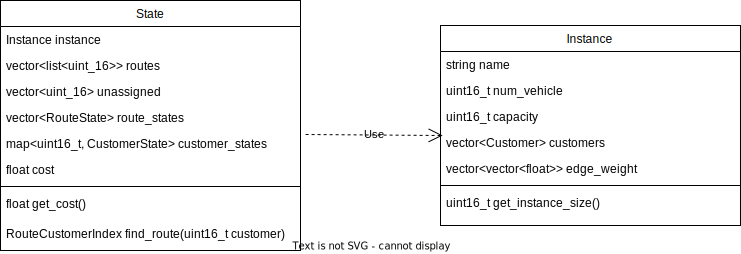
\includegraphics[width=1\textwidth]{figures/core-object.png} 
  % \includesvg[scale=1]{figures/core-object}
  \caption{Đối tượng chính của chương trình} 
  \label{fig:fg_02}
\end{figure}
        \chapter{Ứng dụng ALNS vào CVRPTW}

\begin{figure}[H] % places figure environment here   
  \centering % Centers Graphic
  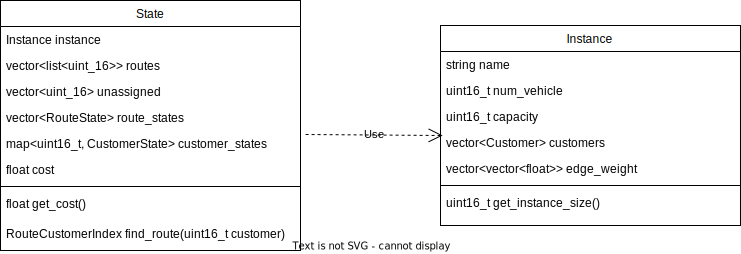
\includegraphics[width=1\textwidth]{figures/core-object.png} 
  % \includesvg[scale=1]{figures/core-object}
  \caption{Đối tượng chính của chương trình} 
  \label{fig:fg_02}
\end{figure}
        \chapter{Thực nghiệm và kết quả}

Trong phần này, chúng ta sẽ xem xét kết quả thực nghiệm thu được khi áp dụng ALNS cho VRPTW với hai tập dữ liệu của Solomon (1987) và Homberger \& Gehring (1999). Ở cả hai tập, các bộ dữ liệu được chia thành 3 loại C, R và RC. Với dữ liệu lớp C, các yêu cầu được phân thành các cụm rõ rệt, lớp R là hoàn toàn ngẫu nhiên và lớp RC là sự kết hợp của hai lớp trên. Tác giả chỉ xem xét các tập từ 100 yêu cầu trở lên (bỏ qua tập Solomon 25, 50 yêu cầu vì nhìn chung số lượng yêu cầu như vậy là quá nhỏ để nhận thấy sự khác biệt khi so sánh ALNS với các thuật toán khác).

\begin{figure}[H] % places figure environment here   
	\label{fig:perf_ct_c1}
	\begin{subfigure}{.3\textwidth}
		\centering
		\includegraphics[width=1\linewidth]{figures/cls_c.png}
		\caption{C-class}
		\label{fig:cls_c}
	\end{subfigure}%
	\begin{subfigure}{.3\textwidth}
		\centering
		\includegraphics[width=1\linewidth]{figures/cls_r.png}
		\caption{R-class}
		\label{fig:cls_r}
	\end{subfigure}
	\begin{subfigure}{.3\textwidth}
		\centering
		\includegraphics[width=1\linewidth]{figures/cls_rc.png}
		\caption{RC-class}
		\label{fig:cls_rc}
	\end{subfigure}
	\caption{Lớp các cấu hình}
\end{figure}

\begin{figure}[H] % places figure environment here   
	\label{fig:perf_ct_c1}
	\begin{subfigure}{.3\textwidth}
		\centering
		\includegraphics[width=1\linewidth]{figures/routes_c101.png}
		\caption{C-class}
		\label{fig:route_c}
	\end{subfigure}%
	\begin{subfigure}{.3\textwidth}
		\centering
		\includegraphics[width=1\linewidth]{figures/routes_r101.png}
		\caption{R-class}
		\label{fig:route_r}
	\end{subfigure}
	\begin{subfigure}{.3\textwidth}
		\centering
		\includegraphics[width=1\linewidth]{figures/routes_rc101.png}
		\caption{RC-class}
		\label{fig:route_rc}
	\end{subfigure}
	\caption{Minh họa lời giải cho các lớp cấu hình}
\end{figure}

Tất cả các thí nghiệm được chạy trên CPU Intel(R) Xeon(R) CPU E5-2680 v4 @ 2.40GHz với Ubuntu 22.04.1 LTS. Mã nguồn được viết bằng ngôn ngữ C++ và được biên dịch bằng GCC 11.4.0 với các tùy chọn tối ưu hóa -O3.

\section{Chất lượng nghiệm}

\subsection{Dữ liệu nhỏ (Solomon)}

Trước tiên, chúng ta bắt đầu với tập dữ liệu Solomon (1987). Với các cấu hình loại C, ALNS cho nghiệm cách nghiệm tốt nhất đã biết trung bình $0.20\%$ và $0.42\%$ cho C1 và C2. 

\begin{table}[caption={Kết quả đo với tập Solomon C \\
  \scriptsize \textit{ins: cấu hình, cost: chi phí thu được với ALNS, nv: số xe được sử dụng, bkcost: chi phí tốt nhất đã biết, bknv: số xe tốt nhất đã biết, gap (\%): khoảng cách so với nghiệm tốt nhất đã biết}}, label=exp:solomonC]
  \begin{adjustbox}{width=1\textwidth}
  \small
  \begin{tabularx}{\textwidth}{lrrrlllrrrll}
  \hline
  \text{ins} & \multicolumn{1}{l}{\text{cost}} & \multicolumn{1}{l}{\text{nv}} & \multicolumn{1}{l}{\text{bkcost}} & \text{bknv} & \text{gap} & \text{ins} & \multicolumn{1}{l}{\text{cost}} & \multicolumn{1}{l}{\text{nv}} & \multicolumn{1}{l}{\text{bkcost}} & \text{bknv} & \text{gap} \\ \hline
  c101 & 828.94 & 10 & 827.30 & 10 & 0.20 & c201 & 591.56 & 3 & 589.10 & 3 & 0.42 \\ \hline
  c102 & 828.94 & 10 & 827.30 & 10 & 0.20 & c202 & 591.56 & 3 & 589.10 & 3 & 0.42 \\ \hline
  c103 & 828.06 & 10 & 826.30 & 10 & 0.21 & c203 & 591.17 & 3 & 588.70 & 3 & 0.42 \\ \hline
  c104 & 824.78 & 10 & 822.90 & 10 & 0.23 & c204 & 590.60 & 3 & 588.10 & 3 & 0.42 \\ \hline
  c105 & 828.94 & 10 & 827.30 & 10 & 0.20 & c205 & 588.88 & 3 & 586.40 & 3 & 0.42 \\ \hline
  c106 & 828.94 & 10 & 827.30 & 10 & 0.20 & c206 & 588.49 & 3 & 586.00 & 3 & 0.43 \\ \hline
  c107 & 828.94 & 10 & 827.30 & 10 & 0.20 & c207 & 588.29 & 3 & 585.80 & 3 & 0.42 \\ \hline
  c108 & 828.94 & 10 & 827.30 & 10 & 0.20 & c208 & 588.32 & 3 & 585.80 & 3 & 0.43 \\ \hline
  c109 & 828.94 & 10 & 827.30 & 10 & 0.20 &  &  &  &  &  &  \\ \hline
  avg & & & & & 0.20 &  &  &  &  & & 0.42 \\ \hline
  \end{tabularx}
  \end{adjustbox}
  \end{table}
  Thí nghiệm được thiết lập có thời gian timeout 1 phút, chạy 5 lần và lấy kết quả tốt nhất. Tập C1 và C2 tương đối nhỏ và đã phân cụm nên trong thực tế thuật toán chạy rất nhanh để ra được nghiệm tối ưu và không có sự khác biệt giữa các lần chạy, trên CPU được thí nghiệm, ALNS mất dưới 1 giây để tìm ra nghiệm tối ưu.


  \begin{table}[caption={Kết quả đo với tập Solomon R1}, label=exp:solomonR1]
    % \begin{adjustbox}{width=1\textwidth}
    \centering
    \begin{tabular}{lrrrll}
    \hline
    instance & \multicolumn{1}{l}{alns best} & \multicolumn{1}{l}{nv} & \multicolumn{1}{l}{bk cost} & bk nv & gap (\%) \\ \hline
    \text{r101} & 1,642.88 & 20 & \text{1,637.70} & 20 & \text{0.32} \\ \hline
    \text{r102} & 1,472.81 & 18 & \text{1,466.60} & 18 & \text{0.42} \\ \hline
    \text{r103} & 1,213.62 & 15 & \text{1,208.70} & 14 & \text{0.41} \\ \hline
    \text{r104} & 976.61 & 11 & \text{971.50} & 11 & \text{0.53} \\ \hline
    \text{r105} & 1,360.78 & 15 & \text{1,355.30} & 15 & \text{0.40} \\ \hline
    \text{r106} & 1,239.37 & 13 & \text{1,234.60} & 13 & \text{0.39} \\ \hline
    \text{r107} & 1,073.60 & \text{12} & \text{1,064.60} & \text{11} & \text{0.85} \\ \hline
    \text{r108} & 944.44 & 10 & \text{932.10} & 10 & \text{1.32} \\ \hline
    \text{r109} & 1,152.38 & 13 & \text{1,146.90} & 13 & \text{0.48} \\ \hline
    \text{r110} & 1,078.59 & 12 & \text{1,068.00} & 12 & \text{0.99} \\ \hline
    \text{r111} & 1,053.50 & 12 & \text{1,048.70} & 12 & \text{0.46} \\ \hline
    \text{r112} & \text{955.68} & 10 & \text{948.60} & \text{10} & \text{0.75} \\ \hline
    avg &  &  &  &  & 0.61 \\ \hline
    \end{tabular}
    % \end{adjustbox}
  \end{table}


  \begin{table}[caption={Kết quả đo với tập Solomon R2}, label=exp:solomonR2]
    % \begin{adjustbox}{width=1\textwidth}
    \centering
    \begin{tabular}{lrrrll}
    \hline
    instance & \multicolumn{1}{l}{alns best} & \multicolumn{1}{l}{nv} & \multicolumn{1}{l}{bk cost} & bk nv & gap (\%) \\ \hline
    r201 & 1,152.96 & \textbf{7} & 1,143.20 & 8 & 0.32 \\ \hline
    r202 & 1,035.32 & \textbf{7} & 1,029.60 & 8 & 0.42 \\ \hline
    r203 & 880.90 & 6 & 870.80 & 6 & 0.41 \\ \hline
    r204 & 743.91 & \textbf{4} & 731.30 & 5 & 0.53 \\ \hline
    r205 & 958.81 & 5 & 949.80 & 5 & 0.40 \\ \hline
    r206 & 883.92 & 5 & 875.90 & 5 & 0.39 \\ \hline
    r207 & 806.31 & 5 & 794.00 & 4 & 0.85 \\ \hline
    r208 & 948.57 & 4 & 701.00 & 4 & 1.77 \\ \hline
    r209 & 717.53 & 5 & 854.80 & 5 & 0.48 \\ \hline
    r210 & 909.32 & \textbf{5} & 900.50 & 6 & 0.99 \\ \hline
    r211 & 1,053.50 & 5 & 746.70 & 4 & 0.46 \\ \hline
    avg &  &  &  &  & 1.38 \\ \hline
    \end{tabular}
    % \end{adjustbox}
  \end{table}

  Tập R1 và R2 có các yêu cầu được tạo hoàn toàn ngẫu nhiên thế nên cũng có nhiều nghiệm chấp nhận được và thuật toán cũng khó bị bẫy ở một nghiệm tối ưu cục bộ. Tuy nhiên, thuật toán cũng mất nhiều thời gian để tìm nghiệm tối ưu hơn do có quá nhiều nghiệm thỏa mãn các ràng buộc. Riêng với tập R2, ALNS đã tìm ra nghiệm với số xe ít hơn nghiệm tốt nhất đã biết mà tổng khoảng cách chỉ chênh lệch nhỏ. 

  \begin{table}[caption={Kết quả đo với tập Solomon RC1}, label=exp:solomonRC1]
    % \begin{adjustbox}{width=1\textwidth}
    \centering
    \begin{tabular}{lrrrll}
    \hline
    instance & \multicolumn{1}{l}{alns best} & \multicolumn{1}{l}{nv} & \multicolumn{1}{l}{bk cost} & bk nv & gap (\%) \\ \hline
    rc101 & 1,623.58 & 16 & 1,619.80 & 15 & 0.23 \\ \hline
    rc102 & 1,461.23 & 14 & 1,457.40 & 14 & 0.26 \\ \hline
    rc103 & 1,266.62 & 11 & 1,258.00 & 11 & 0.69 \\ \hline
    rc104 & 1,136.91 & 10 & 1,132.30 & 10 & 0.41 \\ \hline
    rc105 & 1,518.58 & 16 & 1,513.70 & 15 & 0.32 \\ \hline
    rc106 & 1,376.99 & 13 & 1,372.70 & 12 & 0.31 \\ \hline
    rc107 & 1,211.11 & 12 & 1,207.80 & 12 & 0.27 \\ \hline
    rc108 & 1,118.13 & 11 & 1,114.20 & 11 & 0.35 \\ \hline
    avg &  &  &  &  & 0.36 \\ \hline
    \end{tabular}
    % \end{adjustbox}
  \end{table}

  \begin{table}[caption={Kết quả đo với tập Solomon RC2}, label=exp:solomonRC2]
    % \begin{adjustbox}{width=1\textwidth}
    \centering
    \begin{tabular}{lrrrll}
    \hline
    instance & \multicolumn{1}{l}{alns best} & \multicolumn{1}{l}{nv} & \multicolumn{1}{l}{bk cost} & bk nv & gap (\%) \\ \hline
    rc201 & 1,274.61 & \textbf{8} & 1,261.80 & 9 & 1.02 \\ \hline
    rc202 & 1,099.54 & \textbf{6} & 1,092.30 & 8 & 0.66 \\ \hline
    rc203 & 931.16 & 5 & 923.70 & 5 & 0.81 \\ \hline
    rc204 & 788.66 & 4 & 783.50 & 4 & 0.66 \\ \hline
    rc205 & 1,157.66 & 7 & 1,154.00 & 7 & 0.32 \\ \hline
    rc206 & 1,060.50 & \textbf{6} & 1,051.10 & 7 & 0.89 \\ \hline
    rc207 & 966.08 & 6 & 962.90 & 6 & 0.33 \\ \hline
    rc208 & 785.73 & 4 & 776.10 & 4 & 1.24 \\ \hline
    avg &  &  &  &  & 0.74 \\ \hline
    \end{tabular}
    % \end{adjustbox}
  \end{table}

  Tập RC1 và RC2 chứa các yêu cầu ở các vị trí được phân cụm một cách tương đối (lai giữa tập R và tập C) được đánh giá là tập khó, do các vị trí của yêu cầu đủ ngẫu nhiên để bài toán có nhiều nghiệm chấp nhận được nhưng lại dễ bị bẫy ở nghiệm tối ưu cục bộ khi mà xe đã phụ vụ các yêu cầu ở trong một cụm chỉ cần ta bỏ đi một (vài) yêu cầu "quan trọng" trong cụm là đã nhận được một nghiệm tệ hơn trước khá nhiều. Mặc dù vậy ALNS vẫn tỏ ra hiệu quả khi tìm được nghiệm với chênh lệch trung bình $0.36\%$ và $0.74\%$ cho RC1 và RC2. Ngoài ra, ALNS cũng tìm được nghiệm với số xe ít hơn nghiệm tốt nhất đã biết trong một số cấu hình của tập RC2.
\section{Hiệu năng thuật toán}
Trong phần này chúng ta sẽ xem xét hiệu năng của ALNS. Để thấy rõ sự khác biệt, các đồ thị được trình bày dưới đây là kết quả cho cấu hình với số lượng yêu cầu rất lớn ($1000$ yêu cầu) và số lượng yêu cầu trung bình ($400$ yêu cầu). Ngoài ra, để tránh dài dòng, các đồ thị được thể hiện cho 3 cầu hình C1\_x\_1, R1\_x\_1, RC1\_x\_1 ($x = 10$ cho tập $1000$ yêu cầu, và $x=4$ cho tập $400$ yêu cầu). Hiệu năng của các thuật toán đối với các cấu hình khác là tương tự. Chúng ta sẽ so sánh hiệu năng của ALNS nguyên bản, B-ALNS và một framework rất nổi tiếng trong cộng đồng là \code{Google OR-Tools}. Hiệu năng được so sánh cho cả phiên bản đơn luồng và đa luồng của ALNS.

\subsection{Giá trị hàm mục tiêu}

Trước hết, giá trị hàm mục tiêu theo thời gian được xem xét. Các đồ thị dưới đây cho thấy giá trị hàm mục tiêu theo thời gian khi chạy thuật toán với thời gian chạy 60 giây và được phóng đại để nhìn rõ hơn sự khác biệt trong 10 giây đầu tiên. Đồ thị được chia làm 3 phần tương ứng với 3 cấu hình khác nhau.

\begin{figure}[H] % places figure environment here   
  \label{fig:perf_ct_c1_10}
  \begin{subfigure}{.5\textwidth}
    \centering
    \includegraphics[width=1\linewidth]{figures/cost_time_60s_C1_10_1.png}
    \caption{60s}
    \label{fig:perf_ct_c1_10_60s}
  \end{subfigure}%
  \begin{subfigure}{.5\textwidth}
    \centering
    \includegraphics[width=1\linewidth]{figures/cost_time_10s_C1_10_1.png}
    \caption{10s}
    \label{fig:perf_ct_c1_10_10s}
  \end{subfigure}
  \caption{Giá trị hàm mục tiêu theo thời gian, cấu hình C1\_10\_1}
\end{figure}

\begin{figure}[H] % places figure environment here   
  \label{fig:perf_ct_r1_10}
  \begin{subfigure}{.5\textwidth}
    \centering
    \includegraphics[width=1\linewidth]{figures/cost_time_60s_R1_10_1.png}
    \caption{60s}
    \label{fig:perf_ct_r1_10_60s}
  \end{subfigure}%
  \begin{subfigure}{.5\textwidth}
    \centering
    \includegraphics[width=1\linewidth]{figures/cost_time_10s_R1_10_1.png}
    \caption{10s}
    \label{fig:perf_ct_r1_10_10s}
  \end{subfigure}
  \caption{Giá trị hàm mục tiêu theo thời gian, cấu hình R1\_10\_1}
\end{figure}

\begin{figure}[H] % places figure environment here   
  \label{fig:perf_ct_rc1_10}
  \begin{subfigure}{.5\textwidth}
    \centering
    \includegraphics[width=1\linewidth]{figures/cost_time_60s_RC1_10_1.png}
    \caption{60s}
    \label{fig:perf_ct_rc1_10_60s}
  \end{subfigure}%
  \begin{subfigure}{.5\textwidth}
    \centering
    \includegraphics[width=1\linewidth]{figures/cost_time_10s_RC1_10_1.png}
    \caption{10s}
    \label{fig:perf_ct_rc1_10_10s}
  \end{subfigure}
  \caption{Giá trị hàm mục tiêu theo thời gian, cấu hình RC1\_10\_1}
\end{figure}

\begin{figure}[H] % places figure environment here   
  \label{fig:perf_ct_c1_4}
  \begin{subfigure}{.5\textwidth}
    \centering
    \includegraphics[width=1\linewidth]{figures/cost_time_10s_C1_4_1.png}
    \caption{10s}
    \label{fig:perf_ct_c1_4_10s}
  \end{subfigure}%
  \begin{subfigure}{.5\textwidth}
    \centering
    \includegraphics[width=1\linewidth]{figures/cost_time_1s_C1_4_1.png}
    \caption{1s}
    \label{fig:perf_ct_c1_4_1s}
  \end{subfigure}
  \caption{Giá trị hàm mục tiêu theo thời gian, cấu hình C1\_4\_1}
\end{figure}

\begin{figure}[H] % places figure environment here   
  \label{fig:perf_ct_r1}
  \begin{subfigure}{.5\textwidth}
    \centering
    \includegraphics[width=1\linewidth]{figures/cost_time_10s_R1_4_1.png}
    \caption{10s}
    \label{fig:perf_ct_r1_60s}
  \end{subfigure}%
  \begin{subfigure}{.5\textwidth}
    \centering
    \includegraphics[width=1\linewidth]{figures/cost_time_1s_R1_4_1.png}
    \caption{1s}
    \label{fig:perf_ct_r1_10s}
  \end{subfigure}
  \caption{Giá trị hàm mục tiêu theo thời gian, cấu hình R1\_4\_1}
\end{figure}

\begin{figure}[H] % places figure environment here   
  \label{fig:perf_ct_rc1_4}
  \begin{subfigure}{.5\textwidth}
    \centering
    \includegraphics[width=1\linewidth]{figures/cost_time_10s_RC1_4_1.png}
    \caption{10s}
    \label{fig:perf_ct_rc1_4_10s}
  \end{subfigure}%
  \begin{subfigure}{.5\textwidth}
    \centering
    \includegraphics[width=1\linewidth]{figures/cost_time_1s_RC1_4_1.png}
    \caption{1s}
    \label{fig:perf_ct_rc1_4_1s}
  \end{subfigure}
  \caption{Giá trị hàm mục tiêu theo thời gian, cấu hình RC1\_4\_1}
\end{figure}

Với thời gian chạy lâu, các thuật toán đều chững lại bởi khi đó các tuyến đường đã khá chật chội, việc "sửa chữa" là khó khăn hơn giai đoạn đầu rất nhiều. Nói cách khác, thuật toán bị bẫy trong nghiệm tối ưu cục bộ. Khi chạy thuật toán với thời gian lâu hơn (timeout 10 phút), tác giả nhận thấy hàm mục tiêu không giảm đáng kể nữa. Chính vì thế, thời gian chạy 60 giây được lựa chọn để vừa phù hợp với thực tế và tránh việc chạy quá lâu.

Ta thấy một xu hướng rõ ràng, trong giai đoạn đầu, B-ALNS tăng tốc hiệu năng của ALNS một cách đáng kể. Với tập dữ liệu $1000$ yêu cầu, thời gian chạy dưới 10 giây, B-ALNS đơn luồng cho hiệu năng gần như tương đương với ALNS với 4 luồng. Nghĩa là, B-ALNS tiết kiệm khoảng $75\%$ tài nguyên CPU để đạt kết quả tương đương với ALNS trong thời gian chạy dưới 10 giây. Chưa kể, memory cũng được tiết kiệm một cách đáng kể khi B-ALNS sử dụng 1 luồng thay vì 4 luồng. Khi so sánh với ALNS đơn luồng, B-ALNS đơn luồng cho hiệu năng vượt trội. Đối với tập dữ liệu có số lượng yêu cầu trung bình ($400$ yêu cầu), B-ALNS đơn luồng không có lợi thế so với ALNS đơn luồng, tuy nhiên hiệu năng đa luồng vẫn tốt hơn ALNS. Điều này cho thấy, B-ALNS có thể được sử dụng để giải quyết các bài toán lớn với tài nguyên hạn chế. Với cấu hình $400$ yêu cầu, B-ALNS đa luồng cho hiệu năng bỏ xa ALNS với thời gian chạy dưới $0.2$ giây và luôn tốt hơn trong thời gian chạy dưới $1$ giây. 

Khi so sánh với \code{Google OR-Tools}, ta thấy rằng, \code{Google OR-Tools} cho hiệu năng tốt trong thời gian chạy từ 2 đến 4 giây đầy tiên (tập $1000$ yêu cầu). Tuy nhiên với thời gian chạy dưới 1 giây, \code{Google OR-Tools} không thể cho ra kết quả. Với thời gian chạy lâu hơn, \code{Google OR-Tools} cho hiệu năng không tốt bằng ALNS hay B-ALNS. Với cấu hình $400$ yêu cầu, nhìn chung hiệu năng của B-ALNS cũng như ALNS bỏ xa \code{Google OR-Tools}.

Như vậy đối với các nghiệp vụ yêu cầu một kết quả tốt trong thời gian ngắn, B-ALNS là lựa chọn tốt nhất. Khi tiến hành đo đạc với thời gian chạy dài (timeout lớn hơn 1 phút), tác giả nhận thấy rằng, ALNS là tốt nhất trong các thuật toán được đề cập ở đây. Các kết quả được chỉ ra trong phần trước là giá trị hàm mục tiêu khi sử dụng ALNS nguyên bản.

\subsection{Số xe}

Chúng ta cũng nhận thấy một xu hướng tương tự như khi so sánh hiệu năng của các thuật toán khi sử dụng độ đo là giá trị hàm mục tiêu. B-ALNS cho hiệu năng vượt trội trong giai đoạn đầu. B-ALNS đơn luồng cho hiệu năng tương đương với ALNS với 4 luồng. Với cấu hình lớp R ($1000$ yêu cầu), B-ALNS tiết kiệm được khoảng $30\%$ số xe so với ALNS trong thời gian chạy từ 2 tới 4 giây! Tương tự, với cấu hình $400$ yêu cầu, B-ALNS giảm số xe nhanh hơn đáng kể so với ALNS trong thời gian chạy ngắn (dưới $0.2$ giây).  Việc tiết kiệm hàng trăm xe có ý nghĩa rất lớn trong thực tế. Thường thì chi phí cho một xe (thuê, hoặc mua, nhiên liệu, chi phí cho tài xế, ...) là rất lớn. Việc tiết kiệm số xe sẽ giúp giảm chi phí vận hành của doanh nghiệp một cách đáng kể. 

Với thời gian chạy lâu hơn, đương nhiên chúng ta rất khó để giảm được số xe nữa, vì hầu hết các tuyến đường đến lúc này đã chật chội hơn đáng kể so với giai đoạn đầu.

\begin{figure}[H] % places figure environment here   
  \label{fig:perf_ct_c1_10}
  \begin{subfigure}{.5\textwidth}
    \centering
    \includegraphics[width=1\linewidth]{figures/nv_time_60s_C1_10_1.png}
    \caption{60s}
    \label{fig:perf_ct_c1_10_60s}
  \end{subfigure}%
  \begin{subfigure}{.5\textwidth}
    \centering
    \includegraphics[width=1\linewidth]{figures/nv_time_10s_C1_10_1.png}
    \caption{10s}
    \label{fig:perf_ct_c1_10_10s}
  \end{subfigure}
  \caption{Số xe sử dụng theo thời gian, cấu hình C1\_10\_1}
\end{figure}

\begin{figure}[H] % places figure environment here   
  \label{fig:perf_ct_r1_10}
  \begin{subfigure}{.5\textwidth}
    \centering
    \includegraphics[width=1\linewidth]{figures/nv_time_60s_R1_10_1.png}
    \caption{60s}
    \label{fig:perf_ct_r1_10_60s}
  \end{subfigure}%
  \begin{subfigure}{.5\textwidth}
    \centering
    \includegraphics[width=1\linewidth]{figures/nv_time_10s_R1_10_1.png}
    \caption{10s}
    \label{fig:perf_ct_r1_10_10s}
  \end{subfigure}
  \caption{Số xe sử dụng theo thời gian, cấu hình R1\_10\_1}
\end{figure}

\begin{figure}[H] % places figure environment here   
  \label{fig:perf_ct_rc1}
  \begin{subfigure}{.5\textwidth}
    \centering
    \includegraphics[width=1\linewidth]{figures/nv_time_60s_RC1_10_1.png}
    \caption{60s}
    \label{fig:perf_ct_rc1_60s}
  \end{subfigure}%
  \begin{subfigure}{.5\textwidth}
    \centering
    \includegraphics[width=1\linewidth]{figures/nv_time_10s_RC1_10_1.png}
    \caption{10s}
    \label{fig:perf_ct_rc1_10s}
  \end{subfigure}
  \caption{Số xe sử dụng theo thời gian, cấu hình RC1\_10\_1}
\end{figure}

\begin{figure}[H] % places figure environment here   
  \label{fig:perf_ct_c1_4}
  \begin{subfigure}{.5\textwidth}
    \centering
    \includegraphics[width=1\linewidth]{figures/nv_time_10s_C1_4_1.png}
    \caption{10s}
    \label{fig:perf_ct_c1_4_10s}
  \end{subfigure}%
  \begin{subfigure}{.5\textwidth}
    \centering
    \includegraphics[width=1\linewidth]{figures/nv_time_1s_C1_4_1.png}
    \caption{1s}
    \label{fig:perf_ct_c1_4_1s}
  \end{subfigure}
  \caption{Số xe sử dụng theo thời gian, cấu hình C1\_4\_1}
\end{figure}

\begin{figure}[H] % places figure environment here   
  \label{fig:perf_ct_r1_4}
  \begin{subfigure}{.5\textwidth}
    \centering
    \includegraphics[width=1\linewidth]{figures/nv_time_10s_R1_4_1.png}
    \caption{10s}
    \label{fig:perf_ct_r1_4_10s}
  \end{subfigure}%
  \begin{subfigure}{.5\textwidth}
    \centering
    \includegraphics[width=1\linewidth]{figures/nv_time_1s_R1_4_1.png}
    \caption{1s}
    \label{fig:perf_ct_r1_4_1s}
  \end{subfigure}
  \caption{Số xe sử dụng theo thời gian, cấu hình R1\_4\_1}
\end{figure}

\begin{figure}[H] % places figure environment here   
  \label{fig:perf_ct_rc1}
  \begin{subfigure}{.5\textwidth}
    \centering
    \includegraphics[width=1\linewidth]{figures/nv_time_10s_RC1_4_1.png}
    \caption{10s}
    \label{fig:perf_ct_rc1_4_10s}
  \end{subfigure}%
  \begin{subfigure}{.5\textwidth}
    \centering
    \includegraphics[width=1\linewidth]{figures/nv_time_1s_RC1_4_1.png}
    \caption{1s}
    \label{fig:perf_ct_rc1_4_1s}
  \end{subfigure}
  \caption{Số xe sử dụng theo thời gian, cấu hình RC1\_4\_1}
\end{figure}
        \chapter{Kết luận}
\label{chap:conclusion}

Trong luận văn này, tác giả đã nghiên cứu mô hình toán học, các thuật toán giải lớp các bài toán định tuyến xe, đi sâu vào phương pháp tìm kiếm lân cận rộng. Thuật toán \textit{Tìm kiếm lân cận rộng thích ứng - ALNS} được sử dụng để giải bài toán \textit{Định tuyến xe với ràng buộc tải trọng và khung thời gian - VRPTW}. Tác giả đã đề xuất một hiệu chỉnh giúp tăng hiệu năng của ALNS một cách đáng kể được chỉ ra trong kết quả thực nghiệm. Thuật toán được đặt tên là B-ALNS (\textit{Boosted - Adaptive Large Neighborhood Search - Tìm kiếm lân cận rộng thích ứng tăng tốc}). B-ALNS được đánh giá trên các tập dữ liệu thực tế với số lượng yêu cầu (khách hàng) từ trung bình tới rất lớn cho hiệu năng vượt xa ALNS gốc cũng như framework phổ biến \code{Google OR-Tools}. Điều này gợi ý sử dụng B-ALNS cho các bài toán thực tế yêu cầu chất lượng nghiệm tốt trong thời gian ngắn. Ngoài ra B-ALNS cũng tiết kiệm tài nguyên tính toán (CPU, bộ nhớ) đáng kể so với ALNS gốc.

Mở rộng nghiên cứu, tác giả sẽ tiếp tục cải tiến hiệu chỉnh B-ALNS để thu được nghiệm chất lượng hơn cũng như hiệu năng cao hơn nữa. Thêm vào đó, tác giả tiếp tục nghiên cứu cơ chế thích ứng để "bỏ đi" và "thêm lại" yêu cầu với số lượng hợp lý theo trạng thái của hệ nhằm cải thiện chất lượng nghiệm cũng như tăng hiệu năng.


    \end{content}
    
    \pagenumbering{Roman}
    \setcounter{page}{\numexpr\value{savepage}}

    % References
    \references{}

    
    % Appendix
    %  \begin{appendix}
    %     % In the appendices, use \section{} instead of \chapter{}
    %      \input{appendices/appendix}
    %  \end{appendix}




    % Declaration of authorship
    % \authorshipstatement[pagenumbering=false]
    % \authorshipstatement[pagenumbering=true]
    % \authorshipstatement[pagenumbering=only]
    
    % Consent form for use of plagiarism detection software
    % Not yet required
    % \consentform[pagenumbering=false]
    % \consentform[pagenumbering=true]
    % \consentform[pagenumbering=only]
    
    % Bonus: Wordcount
    % cd %FOLDER WHERE THE .tex FILES ARE IN %
    % clear
    % texcount -total -q -col -sum *.tex
    
\end{document}
